\documentclass[12pt, oneside]{report}

\usepackage[left=2.5cm, top=2.5cm, bottom=2.5cm, right=2.5cm]{geometry}

\usepackage[utf8]{inputenc}
\usepackage[T1]{polski}
\usepackage[polish]{babel}
\usepackage{hyperref}
\usepackage{physics}
\usepackage{graphicx}
\usepackage{amsthm}
\usepackage{enumitem}
\usepackage{mathtools}
\usepackage{amsfonts}

\newtheorem{theorem}{Twierdzenie}
\newtheorem{lemma}{Lemat}
\newtheorem{definition}{Definicja}
\newcommand\Omicron{O}
\DeclarePairedDelimiter\floor{\lfloor}{\rfloor}

\begin{document}  
\thispagestyle{empty}
\begin{titlepage}
    \begin{center}

           \Large
    \textbf{Uniwersytet Jagielloński w Krakowie}\vspace{0.2cm}\\ Wydział Matematyki i Informatyki
               \vspace*{1cm}
               
         \vspace{3cm}
         \Large
          \textbf{Pola Kyzioł}\\\vspace{0.5cm}
         \normalsize Nr albumu: 1092406\\
             \vspace{2cm}
        \Huge
        \textbf{Algorytmy dynamiczne po dekompozycji drzewowej dla problemów grafowych o spójnych rozwiązaniach.}
      
        \vspace{1.5cm}
        \normalsize
        Praca magisterska\\
        na kierunku Informatyka Analityczna\\ \vspace{0.15cm}
        
        \vfill
        \vspace{2cm}
       \begin{minipage}{1\textwidth}
\begin{flushright}
Praca wykonana pod kierunkiem\\
dr hab. Tomasz Krawczyk\\
Instytut Informatyki Analitycznej 
\end{flushright}
\end{minipage}
        
        \vspace{2cm}
        \begin{center}
      Kraków 2019
        \end{center}
    \end{center}
\end{titlepage}

\newpage 
 \thispagestyle{empty}
\vspace{2.5cm}
\begin{flushleft}
\large \textbf{Oświadczenie autora pracy}\vspace{0.6cm}\\
\end{flushleft}

\noindent Świadom odpowiedzialności prawnej oświadczam, że niniejsza praca dyplomowa została napisana przeze mnie samodzielnie i nie zawiera treści uzyskanych w sposób niezgodny z obowiązującymi przepisami.\\

\noindent Oświadczam również, że przedstawiona praca nie była wcześniej przedmiotem procedur związanych z uzyskaniem tytułu zawodowego w wyższej uczelni.
\vspace{2cm}
\begin{center}
\begin{tabular}{lr}
................................~~~~~~~~~~~~~~~~~~~~~~~~~~~~~~~~~~~~~~&
.......................................... \\
{~~~~Kraków, dnia} & {Podpis autora pracy~~~~}
\end{tabular}
\end{center}
\vspace{5cm}
\begin{flushleft}
\large \textbf{Oświadczenie kierującego pracą}
\end{flushleft}

\noindent Potwierdzam, że niniejsza praca została przygotowana pod moim kierunkiem i~kwalifikuje się do przedstawienia jej w postępowaniu o nadanie tytułu zawodowego.
\vspace{2cm}
\begin{center}
\begin{tabular}{lr}
................................~~~~~~~~~~~~~~~~~~~~~~~~~~~~~~~~~~~~~~&
............................................ \\
{~~~~Kraków, dnia} & {Podpis kierującego pracą~~}
\end{tabular}
\end{center}
\vfill

\newpage
\tableofcontents

\newpage
  	\chapter{Dekompozycja drzewowa}
  		\section{Definicja dekompozycji i szerokości drzewowej}

Dekompozycją drzewową grafu $G$ nazywamy parę $\mathcal{T} = (T, \{X_t : t \in V(T)\})$, gdzie $T$ jest drzewem, a $\{X_t : t \in V(T)\}$
zawiera zbiory wierzchołków grafu $G$ i spełnia następujące warunki:
\begin{itemize}
	\item{Dla każdej krawędzi $\{u, v\} \in E(G)$, istnieje węzeł $t \in V(T)$, taki że $u \in X_t$ i $v \in X_t$.}
	\item{Dla każdego wierzchołka $v \in V(G)$, zbiór $\{t \in V(T): v \in X_t \}$ jest poddrzewem drzewa $T$.}
\end{itemize}
Od tej pory wierzchołki grafu wyjściowego $G$ będą nazywane po prostu \emph{wierzchołkami}, natomiast węzły drzewa $T$ będą nazywane \emph{kubełkami}.
\newline\newline
Szerokość drzewowa dekompozycji drzewowej $\mathcal{T}$ jest zdefiniowana następująco: \newline $sd_\mathcal{T} = max_{t \in V(T)} \abs{X_t - 1}$. Natomiast szerokość drzewowa grafu $G$ jest minimalną szerokością drzewową wziętą po wszystkich możliwych dekompozycjach drzewowych $G$: \newline $sd_G = min \{sd_\mathcal{T}: \mathcal{T} \text{ jest dekompozycją drzewową }G\}$.
  		
  		\section{Ładna dekompozycja drzewowa}
Dla uproszczenia posługiwania się dekompozycją drzewową przy definiowaniu algorytmów dynamicznych, będziemy używać tzw. \emph{ładnej dekompozycji drzewowej}, która została po raz pierwszy wprowadzona przez Kloks \cite{kloks}.
\newline\newline
\emph{Ładna dekompozycja drzewowa} $\mathcal{T} = (T, \{X_t\}_{t \in V(T)})$ musi spełniać następujące warunki:
\begin{itemize}
	\item{$T$ jest ukorzenione.}
	\item{Każdy \emph{kubełek} $T$ ma co najwyżej dwoje dzieci.}
	\item{Jeśli \emph{kubełek} $t$ ma dwoje dzieci $p$ i $q$, wtedy $X_t = X_p = X_q$.}
	\item{Jeśli \emph{kubełek} $t$ ma jedno dziecko $p$, to $\abs{X_t} = \abs{X_p} + 1$ \emph{oraz} $X_p \subset X_t$ albo $\abs{X_t} = \abs{X_p} - 1$ \emph{oraz} $X_t \subset X_p$.}
\end{itemize}
Ponieważ w ładnej dekompozycji drzewowej, \emph{kubełki} różnią się od siebie o co najwyżej jeden \emph{wierzchołek}, każde przejście między jednym a drugim \emph{kubełkiem} odpowiada dokładnie jednej operacji na grafie wyjściowym $G$. Każdy \emph{kubełek} ma jeden z następujących pięciu typów:
\begin{itemize}
	\item{\texttt{WPROWADZAJĄCY v} - \emph{kubełek} ten ma o jeden \emph{wierzchołek} więcej niż jego jedyne dziecko: $X_p \cup \{v\} = X_t$. Każdy wierzchołek $v \in V(G)$, ma co najmniej jeden kubełek wprowadzający.}
	\item{\texttt{ZAPOMINAJĄCY v} - \emph{kubełek} o jednym wierzchołku mniej niż jedgo jedyne dziecko: $X_t \cup \{v\} = X_p$. Jego specjalnym reprezentantem jest korzeń. Dla każdego wierzchołka $v \in V(G)$, istnieje dokładnie jeden kubełek zapominający.}
	\item{\texttt{SCALAJĄCY} - jedyny \emph{kubełek} posiadający dwoje dzieci: $X_t = X_p = X_q$, scala dwa podgrafy o przecięciu $X_t$.}
	\item{\texttt{LIŚĆ} - dla $t$ będącego liściem: $X_t = \emptyset$.}
	\item{\texttt{UZUPEŁNIAJĄCY uv} - \emph{kubełek}, który nie pojawił się w pierwotnej definicji ładnej dekompozycji drzewowej, ale ułatwia definiowanie algorytmów operujących na dekompozycjach drzewowych. \emph{Kubełek} uzupełniający wprowadza krawędź $uv \in E(G)$ (uzupełnia krawędziami reprezentację grafu $G$ w drzewie $T$). \emph{Kubełek} $t$ \texttt{UZUPEŁNIAJĄCY} $uv$ zawiera oba \emph{wierzchołki} krawędzi: $u \in X_t$ i $v \in X_t$. Dla każdego $uv$ istnieje dokładnie jeden kubełek uzupełniający i - przyjmując bez straty ogólności $t(u)$ jest przodkiem $t(v)$ (gdzie $t(v)$ to najwyższy \emph{kubełek}, taki że $v \in X_{t(v)}$) - znajduje się on pomiędzy $t(v)$ a \texttt{ZAPOMINAJĄCY v}.}
\end{itemize}

\begin{figure}
\centering
\label{kwadrat}
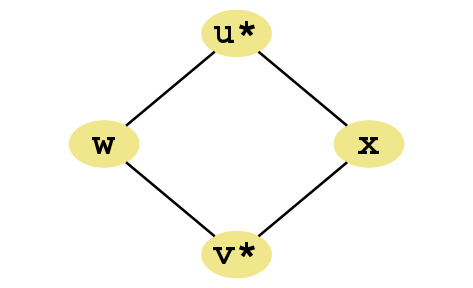
\includegraphics[width=5cm]{square_steiner_tree_standard_graph.png}
\caption{Przykładowy graf $G$.}
\end{figure}

\begin{figure}
\centering
\label{dekompozycja_kwadratu}
\makebox[\textwidth]{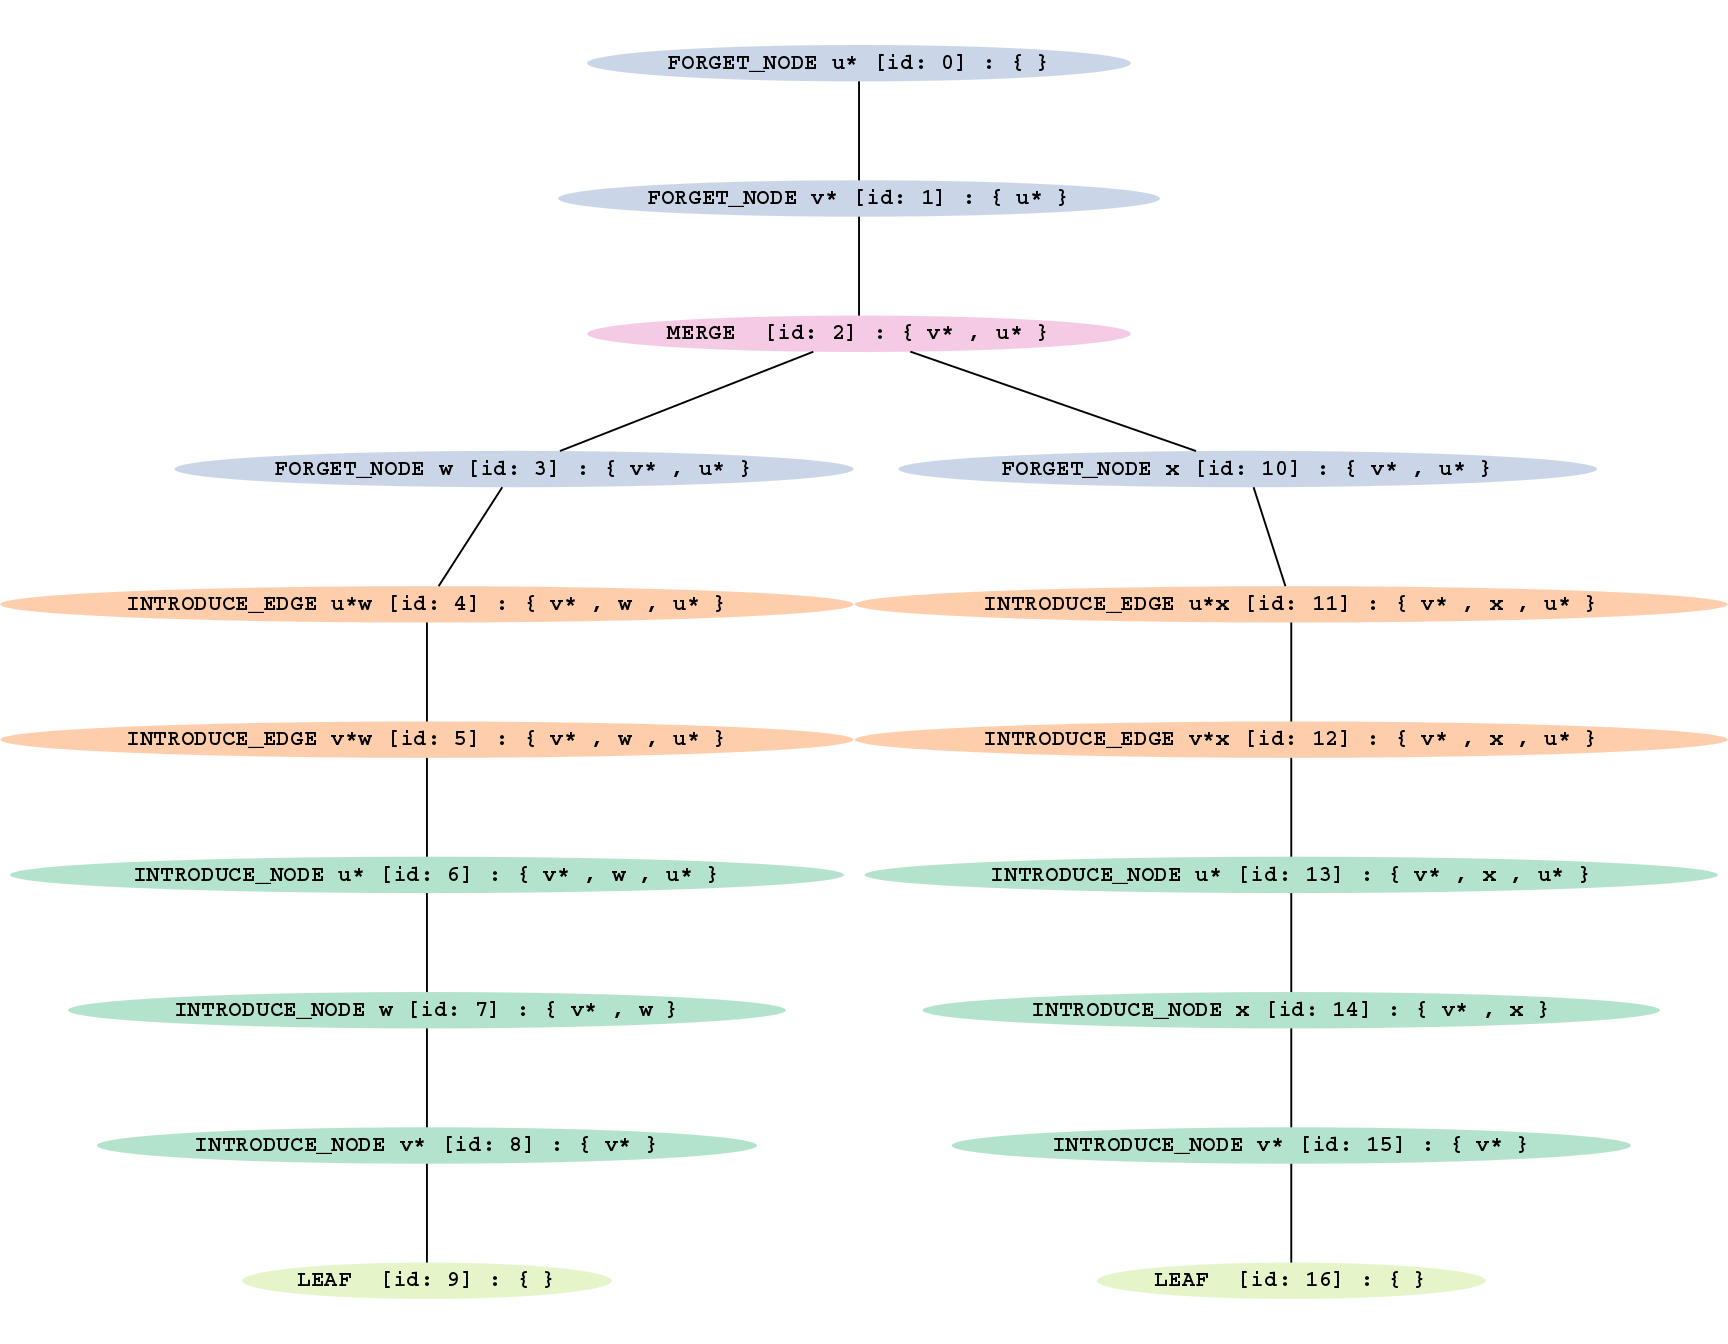
\includegraphics[width=18cm, height=14cm]{square_steiner_tree_standard.png}}
\caption{Ładna dekompozycja drzewowa grafu $G$ z rys. \ref{kwadrat}.}
\end{figure}

Na rysunku \ref{dekompozycja_kwadratu} przedstawiam ładną dekompozycję drzewową dla grafu przedstawionego na rysunku \ref{kwadrat}.

		\section{Obliczanie dekompozycji drzewowej}

Problem obliczania dekompozycji drzewowej należy do klasy problemów FPT. Odkąd Robertson i Seymour \cite{robertson&seymour} wprowadzili w latach osiemndziesiątych definicję dekompozycji drzewowej i jako pierwsi podali parametryzowany algorytm znajdowania dekompozycji drzewowej rozmiaru $\Omicron(k)$ (dla pewnej stałej $k$) o czasie działania $\Omicron(n^{f(k)})$ na grafie $n$-wierzchołkowym ($f(k)$ nigdy nie obliczyli), zostało opublikowanych wiele nowych, wielomianowych algorytmów parametryzowanych o znacznie lepszych złożonościach czasowych. Jednakże Bodlaender \cite{bodlaender} jako pierwszy podał liniowy algorytm znajdowania dekompozycji drzewowej o szerokości $k$ (o ile taka dekompozycja istnieje). 

\begin{theorem}[Bodlaender]
Dla wszystkich $k \in N$ istnieje algorytm działający w czasie liniowym, który dla danego grafu $G = (V, E)$ sprawdza, czy szerokość drzewowa tego grafu wynosi co najwyżej $k$ oraz - jeśli tak - oblicza dekompozycję drzewową $G$ o szerokości drzewowej co najwyżej $k$.  
\end{theorem}

Ponadto Kloks \cite{kloks} pokazał, że dla każdego grafu o szerokości drzewowej $k$ istnieje ładna dekompozycja drzewowa, którą można skonstruować w czasie liniowym od ilości wierzchołków grafu wyjściowego $G$.

\begin{lemma}[Kloks]
\label{kloks}
Każdy graf $G$ o szerokości drzewowej $k$ posiada ładną dekompozycję drzewową o szerokości $k$. Ponadto, jeśli $G$ jest grafem $n$-wierzchołkowym, to istnieje ładna dekompozycja drzewowa grafu $G$ o co najwyżej $4n$ kubełkach.
\end{lemma}

\begin{proof}[Dowód indukcyjny]
Graf $G$ ma szerokość drzewową $k$, wobec czego ma co najmniej $k+1$ wierzchołki. Ponadto każdy graf o szerokości drzewowej $k$ da się striangulować do postaci $k$-drzewa. Triangulacja grafu $G$ do $k$-drzewa opiera się na znalezieniu zrównoważonej dekompozycji drzewowej $\mathcal{T} = (T, \{X_t\}_{t \in V(T)})$, w której dla każdego $t \in V(T)$: $\abs{X_t} = k+1$ oraz dla każdej krawędzi $(t, p) \in E(T)$: $\abs{X_t \cap X_p} = k$, a następnie na dodaniu do $G$ krawędzi między każdą parą wierzchołków $(u, v)$, dla której istnieje kubełek nowo powstałej dekompozycji $t$ : $u \in X_t$ $\wedge$ $v \in X_t$. Algorytm równoważenia dekompozycji drzewowej został przedstawiony przez Bodlaender \cite{bodlaender} i działa on w czasie liniowym. Niech $H$ będzie striangulowanym grafem $G$ o $n$ wierzchołkach. Indukcyjnie można pokazać, że istnieje ładna dekompozycja grafu $H$ o szerokości drzewowej $k$ (w tym twierdzeniu ładna dekompozycja nie zakłada, że liście są puste).
\begin{description}
\item[Dla $n=k+1$,]{możemy wziąć trywialną dekompozycję drzewową, tj. umieścić wszystkie wierzchołki w jednym kubełku.}
\item[Dla $n>k+1$,]{$H$ posiada wierzchołek $v$, którego sąsiedzi tworzą klikę. Niech $H^{\prime}$ będzie grafem otrzymanym z $H$ poprzez usunięcie wierzchołka $v$. Z indukcji dostajemy, że istanieje ładna dekompozycja drzewowa $H^{\prime}$ o co najwyżej $4(n-1)$ kubełkach. Niech $S$ oznacza zbiór sąsiadów wierzchołka $v$. Ponieważ $S$ jest kliką (rozmiaru $k$), musi istnieć kubełek $X_t$ ładnej dekompozycji drzewowej, który zawiera $S$. Rozważmy trzy następujące przypadki dotyczące kubełka $t$:
\begin{enumerate}
\item{$t$ ma dwoje dzieci $p$ i $q$, wobec czego $X_t = X_p = X_q$. Schodzimy w dół drzewa do dowolnego z dzieci i kontynuujemy aż nie znajdziemy się w kubełku $p$ o co najwyżej jednym dziecku.}
\item{$p$ jest liściem. Jeśli $X_p = S$, tworzymy nowy kubełek $a$: $X_a = S \cup \{v\}$, który staje się dzieckiem $p$. Wpp. $X_p \neq S$, niech $z \in X_p \setminus{S}$, $p$ dostaje nowe dziecko $a$: $X_a = X_p \setminus \{z\}$. Ponieważ $S \subset X_p$ i $k = \abs{S} \leq k+1$, $X_a = S$. Dodajemy kolejny kubełek $b$ jako dziecko $a$: $X_b = S \cup {v}$.}
\label{przypadek2}
\item{$p$ ma jedno dziecko $q$. Usuwamy krawędź $(p, q)$ z drzewa. Tworzymy nowy kubełek $a$: $X_a = X_p$ i dodajemy go do drzewa jako dziecko $p$, natomiast $q$ podpinamy jako dziecko $a$. Tworzymy kolejny nowy kubełek $b$: $X_b = X_p$ i podpinamy $b$ jako dziecko $p$ (drugie dziecko). Schodzimy w dół drzewa do kubełka $b$, który jest liściem i postępujemy zgodnie z \ref{przypadek2}. Łatwo zauważyć, że wprowadzimy co najwyżej 4 nowe wierzchołki.} 
\end{enumerate}
Ponieważ dekompozycja drzewowa dla $H^{\prime}$ ma co najwyżej $4(n-1)$ wierzchołki, dekompozycja drzewowa dla $H$ ma co najwyżej $4n$ wierzchołki, co kończy dowód.}
\end{description}
\end{proof}

\begin{lemma}[Kloks]
Dla stałej $k$, mając daną dekompozycję drzewową grafu $G$ o szerokości $k$ i $\Omicron(n)$ wierzchołkach, gdzie $n$ jest liczbą wierzchołków grafu $G$, da się skonstruować ładną dekompozycję drzewową grafu $G$ o szerokości $k$ i co najwyżej $4n$ kubełkach w czasie $\Omicron(n)$. 
\end{lemma}

\begin{proof}
Dowód opiera się na konstrukcji przedstawionej w dowodzie lematu \ref{kloks}. Konstrukcja ta wymaga na wejściu striangulowanego grafu $G$ do postaci $k$-drzewa, triangulacja wymaga czasu liniowego. Szukanie odpowiedniej kolejności usuwania kubełków z $k$-drzewa $H$, czyli takiej w której sąsiedzi usuwanego kubełka indukują klikę, jest również liniowe. Dowód lematu wynika już teraz bezpośrednio z konstrukcji przedstawionej w dowodzie lematu \ref{kloks}.
\end{proof}

\newpage
  	\chapter{Klasyczne algorytmy dynamiczne}
    	\section{Drzewo Steinera}

Niniejszy algorytm został przedstawiony w \cite{parametrized_algorithms}. Mamy dany nieskierowany graf $G$ oraz zbiór wierzchołków $K$ będący podzbiorem $V(G)$, $K \subset V(G)$. Wierzchołki te nazywane są terminalami.
Naszym zadaniem jest znalezienie dla grafu $G$ takiego jego spójnego podgrafu $H$, który zawiera wszystkie terminale i jego rozmiar jest minimalny.
Zakładamy, że mamy daną ładną dekompozycję drzewową grafu wyjściowego $G$ : $\mathcal{T} = (T, \{X_t\}_{t \in V(T)})$. Dodatkowo, dla uproszczenia samego algorytmu, przyjmujemy, że każdy \emph{kubełek} zawiera przynajmniej jeden terminal. Możemy to łatwo osiągnąć - wybieramy dowolny wierzchołek ${v*}$ będący terminalem (terminale będą dla ułatwienia dodatkowo oznaczane przez *) i dodajemy go do każdego kubełka, usuwamy $\texttt{WPROWADZAJĄCY v}$ i $\texttt{ZAPOMINAJĄCY v}$, własność ładnej dekompozycji drzewowej jest zachowana z tą małą modyfikacją, że liście i korzeń nie są puste.
\newline
Zanim przejdziemy do zdefiniowania algorytmu dynamicznego dla problemu Steinera, wprowadźmy kilka dodatkowych oznaczeń.
Dla kubełka $t$, definiujemy:
\begin{description}
\item[$V_t:$]{suma wszystkich kubełków w poddrzewie ukorzenionym w $t$, włączając $X_t$, inaczej mówiąc wszystkie wierzchołki grafu wyjściowego $G$, które pojawiły się w danym poddrzewie}
\item[$E_t:$]{wszystkie krawędzie $(u, v)$, które zostały zrealizowane w poddrzewie ukorzenionym w $t$, czyli dla których istnieje kubełek $p$: $u \in X_p$ $\wedge$ $v \in X_p$} 
\item[$G_t = $]{$(V_t, E_t)$}
\end{description}

Niech $H$ będzie szukanym drzewem Steinera łączącym wszystkie terminale $K$, a $t$ jednym z kubełków $\mathcal{T}$. Przecięcie $H$ i $G_t$ tworzy las $F$, który nigdy nie jest pusty, ponieważ zawiera przynajmniej jeden wierzchołek $v*$ wprowadzony na początku do każdego kubełka. Szukane $H$ jest spójne oraz $X_t$ zawiera terminal, co implikuje, że każde drzewo należące do $F$ musi przecinać $X_t$. Ponadto każdy terminal z $K \cap V_t$ musi należeć do jednego z drzew $F$ - każdy terminal musi należeć do $F$ od momentu pojawienia się w $V_t$. Żeby utrzymać powyższe niezmienniki, trzeba w każdym kubełku rozważać wszystkie możliwe przecięcia $X_t$ z $V(F)$: $X \subset{X_t}$ oraz wszystkie partycje $X$: $\mathcal{P}$ odpowiadające drzewom (komponentom) $F$ - oznaczonym jako $C_1, \dots, C_z$ - i wybierać tylko te, które spełniają następujące warunki: 
\begin{enumerate}
\item{$K \cap V_t \subseteq V(F)$, $F$ zawiera wszystkie dotychczas wprowadzone terminale}
\item{$V(F) \cap X_t = X$, $X$ reprezentuje w danym kubełku to, co bierzemy do drzewa Steinera}
\item{dla wierzchołków należących do przecięcia $V(F) \cap X_t$, $\mathcal{P} = \{\mathcal{P}_1, \dots, \mathcal{P}_z\}$ reprezentuje dokładnie ich przynależność do poszczególnych spójnych komponentów $F$, gdzie dla każdego $y \in \{1, \dots, z\}$: $\mathcal{P}_y = V(C_y) \cap X_t$}
\end{enumerate}
Dla każdej trójki $(t, X, \mathcal{P})$ trzymamy w $c[t][X][\mathcal{P}]$ rozmiar (liczbę krawędzi) najmniejszego $F$ w $G_t$, dla którego powyższe warunki są spełnione (własność optymalnej podstruktury). Jeśli dana trójka nie spełnia wszystkich warunków $c[t][X][\mathcal{P}] = \infty$. Musimy na bieżąco śledzić partycję $\mathcal{P}$, ponieważ może się ona zmieniać wraz z każdym nowo przetwarzanym kubełkiem. Kubełki typu \texttt{SCALAJĄCY} lub \texttt{UZUPEŁNIAJĄCY uv} mogą zepsuć wcześniej poprawną partycję, tworząc cykl. Wynik końcowy odpowiada wartości $c[r][\{v*\}][\{\{v*\}\}]$, gdzie $r$ jest korzeniem. Poniżej prezentuję formuły rekurencyjne obliczania wartości $c$ ze względu na typ kubełka $t$. Dla wszystkich nie wymienionych przypadków, $c$ przyjmuje wartość $\infty$. \newline

\texttt{LIŚĆ} - każdy liść odpowiada następującemu przypadkowi:
$$c[t][\{v*\}][\{\{v*\}\}] = 0$$

\texttt{WPROWADZAJĄCY u} - w związku z tym, że $t$ jest \texttt{WPROWADZAJĄCY}, przyjmijmy następujące oznaczenia $X_t = X_{t^{\prime}} \cup u$, gdzie $t^{\prime}$ jest dzieckiem $t$. Zauważmy, że $u$ nie należał do żadnego z kubełków - przodków $t$, wobec czego krawędzie incydentne z $u$ nie zostały jeszcze wprowadzone poprzez wierzchołki \texttt{UZUPEŁNIAJĄCE} i $u$ jest wierzchołkiem izolowanym. Warunki, które muszą być spełnione:
\begin{enumerate}[label=(\roman*)]
\item $u$ jest izolowany
\item jeśli $u$ jest terminalem, musi się znaleźć w $X$
\item $u$ jako wierzchołek izolowany musi mieć swój własny, jednoelementowy komponent w $\mathcal{P}$
\end{enumerate}
Jeśli któryś z powyższych warunków nie jest spełniony, $c[t][X][\mathcal{P}] = \infty$, wpp. 
\[
c[t][X][\mathcal{P}] =  
\left \{
  \begin{tabular}{ccc}
  $c[t^{\prime}][X \setminus \{u\}][\mathcal{P} \setminus \{\{u\}\}]$ & jeśli $u \in X$,\\
  $c[t^{\prime}][X][\mathcal{P}]$ & wpp.
  \end{tabular}
\right. 
\]
\newline

\texttt{UZUPEŁNIAJĄCY uw} - iterując się po wszystkich trójkach $(t, X, \mathcal{P})$ mamy do czynienia z 3 przypadkami, które musimy rozpatrzeć osobno:

\begin{enumerate}
\item \label{notinx} $u \notin X \lor w \notin X$
\item \label{notinthesamecomponent} $u \in X \land w \in X$ oraz $u$ i $w$ są w różnych komponentach $\mathcal{P}$ ($u \in \mathcal{P}_i$, $w \in \mathcal{P}_j$, $i \neq j$)
\item \label{edgepossible} $u \in X \land w \in X$ oraz $u$ i $w$ są w tych samych komponentach $\mathcal{P}$ ($u,w \in \mathcal{P}_i$)
\end{enumerate} 
W przypadkach \ref{notinx} oraz \ref{notinthesamecomponent} krawędź $uw$ nie może należeć do rozwiązania. Natomiast w przypadku \ref{edgepossible} mamy spełnione warunki, by włączyć krawędź do rozwiązania, mamy zatem dwie możliwości - albo ją bierzemy, albo nie. Jeśli nie dorzucamy krawędzi do naszego aktualnego rozwiązania, przepisujemy częściowy wynik z $t^{\prime}$ dla tej samej partycji. W przeciwnym przypadku, nowo dodawana krawędź musiała połączyć dwa rozłączne bloki partycji $t^{\prime}$. Ponieważ optymalizujemy po rozmiarze częściowego wyniku, iterujemy się po wszystkich partycjach $\mathcal{P}^{\prime}$ kubełka $t^{\prime}$, gdzie $u$ ($\in \mathcal{P}_i$) i $w$ ($\in \mathcal{P}_j$) nie należą do tego samego komponentu ($i \neq j$), inaczej powstałby cykl, ale po połączeniu $\mathcal{P}_i$ z $\mathcal{P}_j$ dają partycję $\mathcal{P}$. Możemy to zapisać następująco:
$$c[t][X][\mathcal{P}] = \min \big\{ \min\limits_{\mathcal{P}^{\prime}} c[t^{\prime}][X][\mathcal{P}^{\prime}] + 1, \quad c[t^{\prime}][X][\mathcal{P}] \big\}$$

\texttt{ZAPOMINAJĄCY u} - niech $X_t = X_{t^{\prime}} \setminus \{u\}$. Wierzchołek $u$ może być incydentny z częściowym rozwiązaniem, wtedy trzeba popatrzeć na te partycje $\mathcal{P^{\prime}}$ kubełka $t^{\prime}$, które go zawierają, a po jego usunięciu dają nam $\mathcal{P}$. Jednakże tylko te, w których nie jest on singletonem, w przeciwnym przypadku nasze częściowe rozwiązanie nigdy nie stałoby się spójnym drzewem Steinera (wszystkie krawędzie incydentne z zapominanym wierzchołkiem są wprowadzane przed jego zapomnieniem i tylko wtedy mogą one zostać dodane do rozwiązania). Iterujemy się po wszystkich $\mathcal{P^{\prime}}$ otrzymanych z $\mathcal{P}$ poprzez dodanie $u$ do jednego z już istniejących bloków, biorąc minimum. Jednocześnie musimy pamiętać, że wierzchołek $u$ może nie należeć do końcowego rozwiązania, wtedy możemy przepisać wynik dla $t^{\prime}$, nie zmieniając parametrów. Kluczową obserwacją dla tego przypadku jest fakt, że jeśli $u$ był terminalem, nie istnieją częściowe rozwiązania dla $t^{\prime}$ nie uwzględniające $u$ (tzn. ich wynikiem jest $\infty$).
$$c[t][X][\mathcal{P}] = \min \big\{ \min\limits_{\mathcal{P}^{\prime}} c[t^{\prime}][X \cup \{u\}][\mathcal{P}^{\prime}], \quad c[t^{\prime}][X][\mathcal{P}] \big\}$$

\texttt{SCALAJĄCY} - kubełek scalający ma zawsze dwoje dzieci, dla których $X_t = X_{t_1} = X_{t_2}$. Dla tego typu kubełków musimy połączyć dwa częściowe rozwiązania - jedno pochodzące z poddrzewa $G_{t_1}$, drugie z poddrzewa $G_{t_2}$. Poniżej znajduje się klika spostrzeżeń kluczowych dla obliczania nowego częściowego rozwiązania:
\begin{enumerate}[label=(\alph*)]
\item $V_{t_1} \cap V_{t_2} = X$
\item $E_{t_1} \cap E_{t_2} = \emptyset$, ponieważ krawędzie wprowadzane są najpóźniej jak to możliwe, tj. przed kubełkami typu \texttt{ZAPOMINAJĄCY}. Zakładając nie wprost, że istnieje krawędź $uw$ zarówno w $E_{t_1}$ jak i w $E_{t_2}$, muszą również istnieć dwa kubełki - bez straty ogólności - \texttt{ZAPOMINAJĄCY u}, jeden w jednym poddrzewie, drugi w drugim poddrzewie lub naddrzewie (w zależności od tego, czy dla drugiego poddrzewa \texttt{ZAPOMINAJĄCY u} jest przodkiem \texttt{ZAPOMINAJĄCY w}). W obu przypadkach dostajemy sprzeczność, ponieważ dla każdego wierzchołka $u$ może istnieć tylko jeden \texttt{ZAPOMINAJĄCY u} (z definicji dekompozycji drzewowej).
\item Połączenie $G_{t_1}$ z $G_{t_2}$ może zawierać cykl. By uniknąć cykli autorzy algorytmu wprowadzają pomocniczą strukturę $G_{\mathcal{P}}$, która jest lasem o zbiorze wierzchołków $X$ oraz której drzewa korespondują z podziałem $\mathcal{P}$. Problem łączenia dwóch rozwiązań częściowych (dla $t_1$ oraz dla $t_2$) sprowadza się do problemu łączenia dwóch lasów $G_{\mathcal{P}_1} \cup G_{\mathcal{P}_2}$. Zauważmy, że z perspektywy wyliczania poprawnego rozwiązania dla kubełka $t$, nie jest ważne, jaki kształt mają poszczególne drzewa, istotny jest fakt, że drzewo jest grafem spójnym (między dowolną parą wierzchołków do niego należących, istnieje ścieżka).
\end{enumerate}

\begin{figure}
\centering
\label{find_n_union}
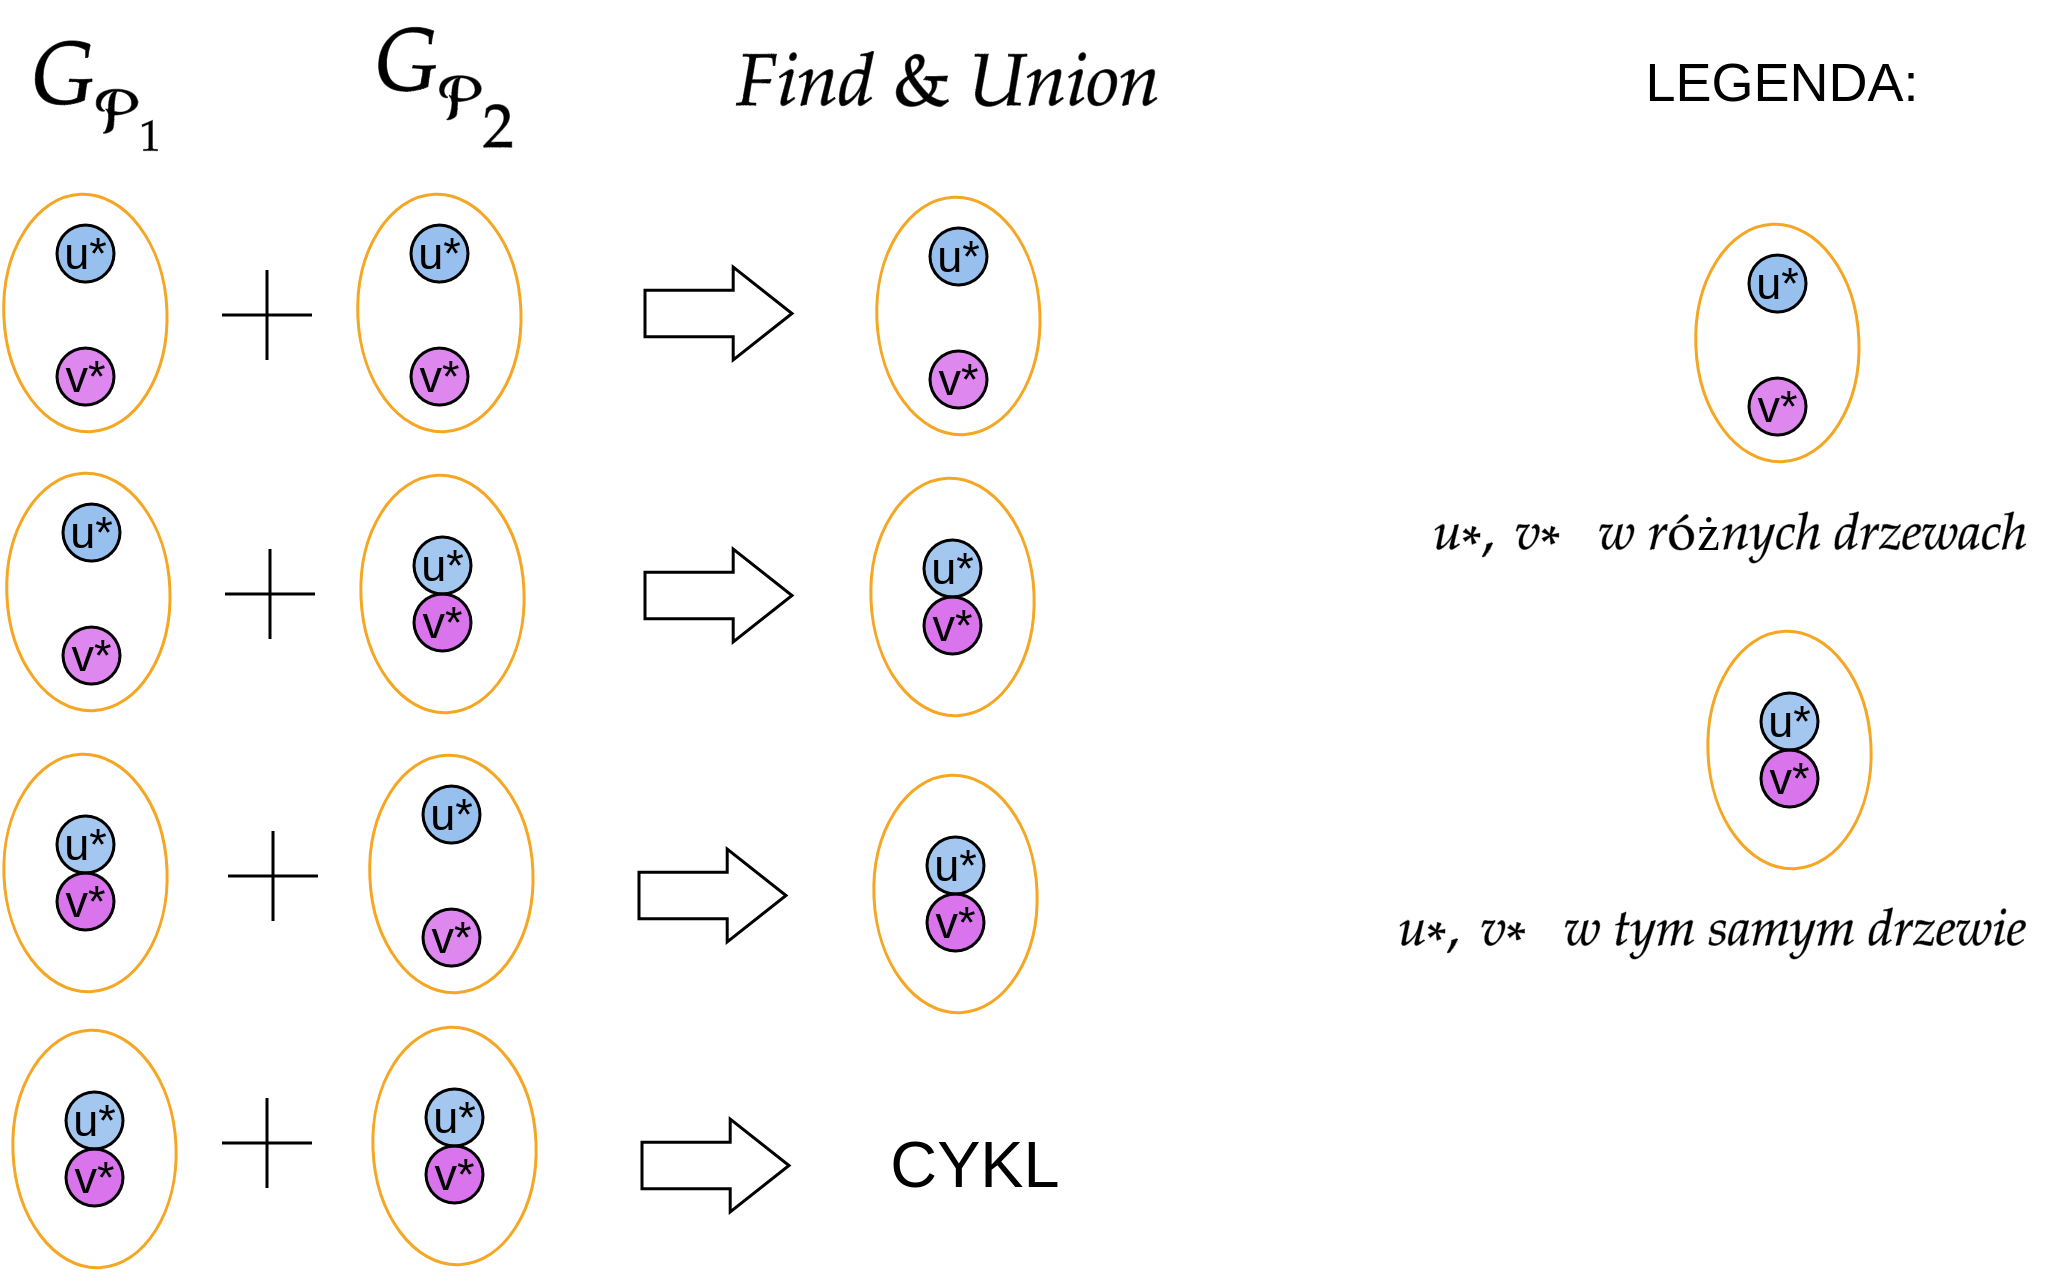
\includegraphics[width=16cm]{find_n_union7.png}
\caption{Rezultaty otrzymane w wyniku połączenia poszczególnych lasów $G_{\mathcal{P}_1}$, $G_{\mathcal{P}_2}$ w kubełku \texttt{SCALAJĄCYM} z rys. \ref{dekompozycja_kwadratu}.}
\end{figure}

Warunki, które muszą zostać spełnione przy scalaniu dwóch rozwiązań są następujące:
\begin{enumerate}[label=(\roman*)]
\item $G_{\mathcal{P}_1} \cup G_{\mathcal{P}_2}$ nie zawiera cyklu.
\item $G_{\mathcal{P}_1} \cup G_{\mathcal{P}_2}$ odpowiada $G_{\mathcal{P}}$ z dokładnością do kształtu poszczególnych drzew. 
\end{enumerate}
W implementacji powyższego algorytmu do reprezentowania problemu łączenia lasów $G_{\mathcal{P}_1}$, $G_{\mathcal{P}_2}$ wykorzystałam strukturę zbiorów rozłącznych z łączeniem według rangi i kompresją ścieżek. Dzięki niej łatwo wykryć cykl oraz zbadać, które wierzchołki są w tych samych, spójnych komponentach $\mathcal{P}$. Rysunek \ref{find_n_union} przedstawia wszystkie możliwe lasy $G_{\mathcal{P}_1}$, $G_{\mathcal{P}_2}$ dla kubełka \texttt{SCALAJĄCEGO} z rysunku \ref{dekompozycja_kwadratu} wraz z rezultatami połączenia lasów.
Końcowe rozwiązanie dla kubełka \texttt{SCALAJĄCEGO} wyliczamy na podstawie poniższego wzoru:
$$c[t][X][\mathcal{P}] = \min \limits_{\mathcal{P}_1, \mathcal{P}_2} c[t_1][X][\mathcal{P}_1] + c[t_2][X][\mathcal{P}_2]$$

Przedstawione zostały formuły rekurencyjne dla wszystkich typów kubełków. Przejdźmy zatem do wyliczenia złożoności czasowej standardowego algorytmu dynamicznego po dekompozycji drzewowej dla problemu drzewa Steinera. Poniżej znajdują się istotne spostrzeżenia:
\begin{itemize}
\item Każdy kubełek ma co najwyżek $k+2$ wierzchołki.
\item Wszystkich $X \subseteq X_t$ jest $2^{\abs{X_t}}$ a zatem nie więcej niż $2^{k+2}$.
\item Wszystkich partycji $X$ jest $\abs{X}^{\abs{X}}$ a zatem nie więcej niż $(k+2)^{k+2}$
\item Dla każdego kubełka mamy $2^{k+2} \cdot (k+2)^{k+2} = k^{\Omicron(k)}$.
\item Wartości dla każdego kubełka wyliczamy w czasie $(k^{\Omicron(k)})^2$.
\end{itemize}
 
\begin{theorem}
Mając dany $n$-wierzchołkowy graf $G$ razem ze zbiorem terminali $K \subseteq V(G)$ oraz dekompozycją drzewową o szerokości drzewowej nie większej niż $k$, można wyliczyć rozmiar minimalnego drzewa Steinera w czasie $k^{\Omicron(k)} \cdot n$. 
\end{theorem}

    	\section{Cykl Hamiltona}
    	
Mamy dany graf $G=(V, E)$. Spacer definiujemy jako naprzemienną sekwencję wierzchołków należących do $V(G)$ i krawędzi należących do $E(G)$, której początkiem i końcem są wierzchołki oraz w której każda występująca krawędź jest incydentna z wierzchołkiem poprzedzającym i następującym. Ścieżką nazywamy spacer, w którym wierzchołki się nie powtarzają. Pytamy, czy istnieje taka ścieżka $H$, która zaczyna i kończy się w tym samym wierzchołku (problem decyzyjny). Zakładamy, że mamy daną ładną dekompozycję drzewową lekko zmodyfikowanego grafu $G^{\prime}$ : $\mathcal{T} = (T, \{X_t\}_{t \in V(T)})$. Modyfikacja polega na tym, że kopiujemy wierzchołek $v$, będący w korzeniu dekompozycji drzewowej grafu $G$ (\texttt{ZAPOMINAJĄCY v}) wraz z jego krawędziami, tj. dla z każdej krawędzi $uv \in E(G)$, dostajemy dwie krawędzie $uv_1$ i $uv_2$, gdzie $v_1$ jest byłym wierzchołkiem $v$, a $v_2$ jego kopią. $\mathcal(T)$ nie zawiera kubełków \texttt{ZAPOMINAJĄCY $v_1$} oraz \texttt{ZAPOMINAJĄCY $v_2$}. Problem szukania cyklu Hamiltona modyfikujemy do problemu szukania ścieżki Hamiltona o końcach $v_1$ i $v_2$.
\newline\newline
Niech $H$ będzie szukanym cyklem Hamiltona. Przecięcie $H$ i $G_t$ składa się z wielu rozłącznych i wierzchołkowo, i krawędziowo ścieżek (również jednoelementowych, będących wierzchołkami izolowanymi), oznaczmy je jako $F$. Przecięcie to poza liśćmi nigdy nie jest puste, ponieważ wszystkie wprowadzone wierzchołki muszą należeć do częściowego rozwiązania. Szukane $H$ jest spójne, co implikuje, że każda ścieżka $C_1, \ldots, C_z$ z $F$ przecina $X_t$. Ponadto musi ona przecinać $X_t$ oboma swoimi końcami, wpp. nie dostalibyśmy spójnego rozwiązania końcowego. Biorąc pod uwagę powyższe wymagania, dostajemy że dla każdej pary ($X_t$, $F$), możemy utworzyć trzy klasy wierzchołków należących do $X_t$ (rys. \ref{hamiltonian}):
\begin{itemize}
\item wierzchołki izolowane w $F$ (o stopniu $0$)
\item wierzchołki będące końcami ścieżek $C_1, \ldots, C_z$ (o stopniu $1$)
\item wierzchołki należące do ścieżek $C_1, \ldots, C_z$ i nie będące ich końcami (o stopniu $2$)
\end{itemize}

\begin{figure}
\centering
\label{hamiltonian}
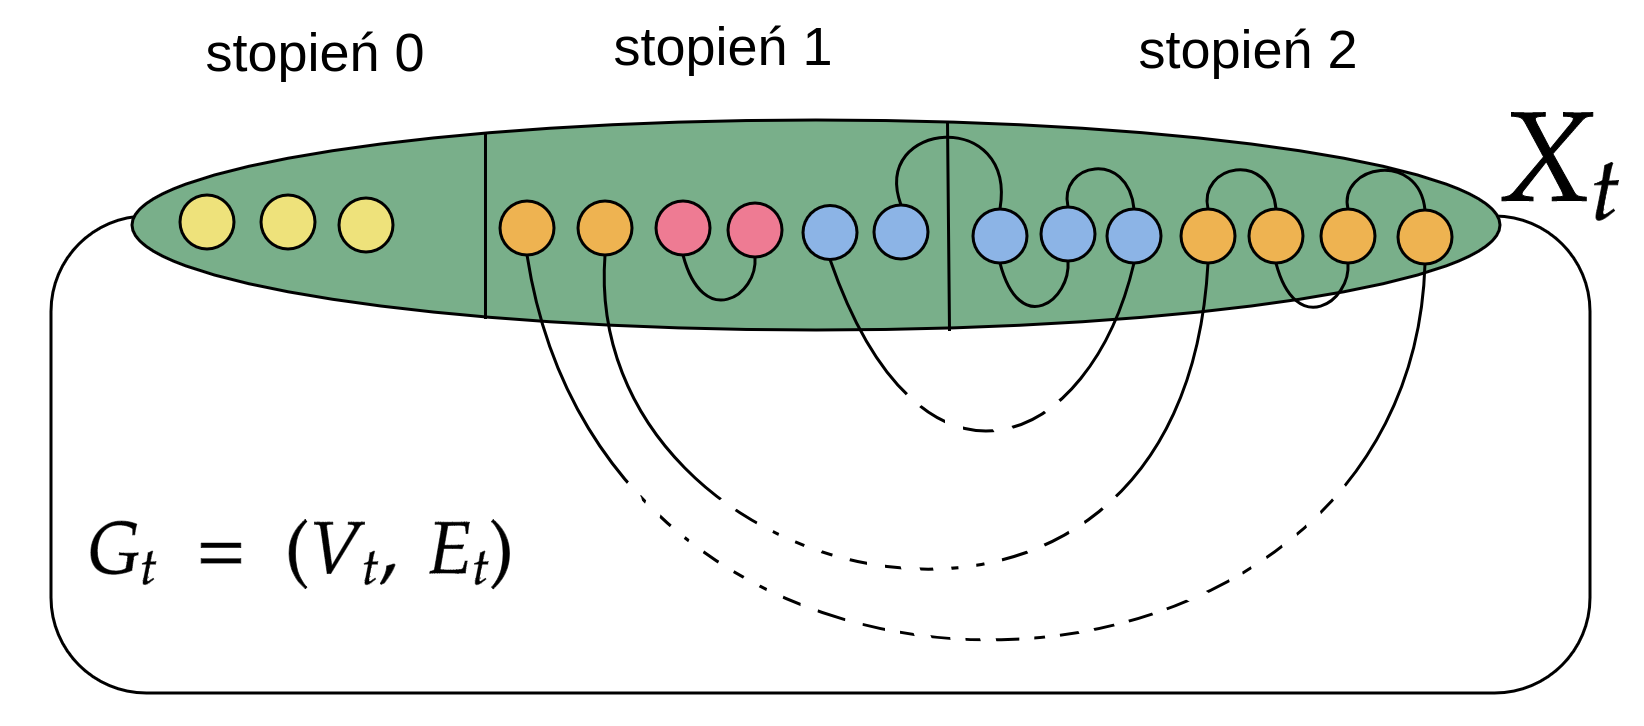
\includegraphics[width=16cm]{hamiltonian3.png}
\caption{Jedno z możliwych rozwiązań częściowych problemu znajdowania ścieżki Hamiltona dla kubełka $t$.}
\end{figure}

By utrzymać powyższe niezmienniki, w każdym kubełku $t$ musimy rozważyć wszystkie możliwe podziały zbioru $X_t$ na trzy podzbiory $\mathcal{D} = (X_{t\_0}$, $X_{t\_1}$, $X_{t\_2})$, odpowiadające stopniom wierzchołków, które się w nich znajdują. Ponadto by w kubełkach \texttt{SCALAJĄCY} oraz \texttt{UZUPEŁNIAJĄCY uw}, nie otrzymać cyklu, musimy się przeiterować po wszystkich możliwych skojarzeniach $M$ wierzchołków ze zbioru $X_{t\_1}$. Rozwiązanie częściowe jest poprawne, jeśli spełnione są następujące warunki:
\begin{enumerate}
\item $V(F) = V_t$ (wszystkie wierzchołki muszą należeć do rozwiązania)
\item $u \in X_{t\_i}$ $\Leftrightarrow$ $u \in X_t$ i wierzchołek $u$ ma stopień $i$ w $F$
\item $\abs{X_{t\_1}} \equiv 0 \mod 2$
\item $u$ jest skojarzone z $w$ (${u, w} \in M$) $\Leftrightarrow$ $u \in X_{t\_1} \wedge w \in X_{t\_1} \wedge \exists y: u \in C_y \wedge w \in C_y$ ($u$ i $w$ są końcami ścieżki $C_y$) 
\end{enumerate}  

Dla każdej trójki $(t, \mathcal{D}, M)$ trzymamy w $c[t][\mathcal{D}][M]$ $0$ lub $1$ w zależności od tego, czy powyższe warunki są spełnione. Musimy na bieżąco śledzić skojarzenie $M$, ponieważ kubełki typu \texttt{SCALAJĄCY} oraz \texttt{UZUPEŁNIAJĄCY uw} mogą utworzyć cykl. Wynik końcowy odpowiada wartości $c[r][(\emptyset, \{v_1, v_2\}, \emptyset)][\{v_1, v_2\}]$, gdzie $r$ jest korzeniem. Poniżej prezentuję formuły rekurencyjne obliczania wartości $c$ ze względu na typ kubełka $t$.
\newline\newline
\texttt{LIŚĆ} - każdy liść odpowiada następującemu przypadkowi:
$$c[t][(\emptyset, \emptyset, \emptyset)][\emptyset] = 1$$

\texttt{WPROWADZAJĄCY u} - zauważmy, że w momencie dodawania wierzchołka do $F$ jego stopień musi wynosić $0$, ponieważ żadna z incydentnych do niego krawędzi nie została jeszcze wprowadzona:

\[
c[t][(X_{t\_0}, X_{t\_1}, X_{t\_2})][M] =  
\left \{
  \begin{tabular}{ccc}
  $c[t^{\prime}][(X_{t\_0} \setminus \{u\}, X_{t\_1}, X_{t\_2})][M]$ & jeśli $u \in X_{t\_0}$,\\
  $0$ & wpp.
  \end{tabular}
\right. 
\]

\texttt{ZAPOMINAJĄCY u} - wszystkie krawędzie incydentne do zapominanego wierzchołka zostały już wprowadzone, wobec czego zapominany wierzchołek musi mieć stopień $2$ w $F$:

$$c[t][(X_{t\_0}, X_{t\_1}, X_{t\_2})][M] = c[t^{\prime}][(X_{t\_0}, X_{t\_1}, X_{t\_2} \cup \{u\})][M]$$

\texttt{UZUPEŁNIAJĄCY uw} - dodawanie krawędzi incydentnej do wierzchołka zwiększa jego stopień o $1$, wobec czego możemy dodawać krawędź, jeśli $u \in X_{t\_0} \vee u \in X_{t\_1}$ oraz $w \in X_{t_0} \vee w \in X_{t\_1}$. Nie jest to jednak warunek wystarczający, ponieważ nie gwarantuje nam, że nie dostaniemy cyklu. Jeśli $u \in X_{t\_1} \wedge w \in X_{t\_1}$ oraz $\exists m : m \in M \wedge u \in m \wedge w \in m$, nie możemy wziąć krawędzi $uw$. Niezależnie od tego, czy krawędź może zostać dodana do rozwiązania, czy nie, dla każdej trójki $(t, \mathcal{D}, M)$ możemy jej nie brać, dlatego bierzemy alternatywę $c[t^{\prime}][(X_{t\_0}, X_{t\_1}, X_{t\_2})][M]$ i poniższych wartości:

\[
c[t][(X_{t\_0}, X_{t\_1}, X_{t\_2})][M] =  
\left \{
  \begin{tabular}{ccc}
  jeśli $u \in X_{t\_1} \wedge w \in X_{t\_1}$:\\
  $c[t^{\prime}][(X_{t\_0} \cup \{u, w\}, X_{t\_1} \setminus \{u, w\}, X_{t\_2})][M \cup \{u, w\}]$\\
  \\
  jeśli $u \in X_{t\_1} \wedge w \in X_{t\_2}$:\\
  $c[t^{\prime}][(X_{t\_0} \cup \{u\}, X_{t\_1} \setminus \{u\} \cup \{w\}, X_{t\_2} \setminus \{w\})][M \cup \{u, w\}]$\\
  \\
  jeśli $u \in X_{t\_2} \wedge w \in X_{t\_1}$:\\
  $c[t^{\prime}][(X_{t\_0} \cup \{w\}, X_{t\_1} \setminus \{w\} \cup \{u\}, X_{t\_2} \setminus \{u\})][M \cup \{u, w\}]$\\
  \\
  jeśli $u \in X_{t\_2} \wedge w \in X_{t\_2}$:\\
  $c[t^{\prime}][(X_{t\_0}, X_{t_1} \cup \{u, w\}, X_{t\_2} \setminus \{u, w\})][M \cup \{u, w\}]$\\
  \\  
  $0$ wpp.\\
  \end{tabular}
\right. 
\]

\begin{figure}
\centering
\label{hamiltonian_merge}
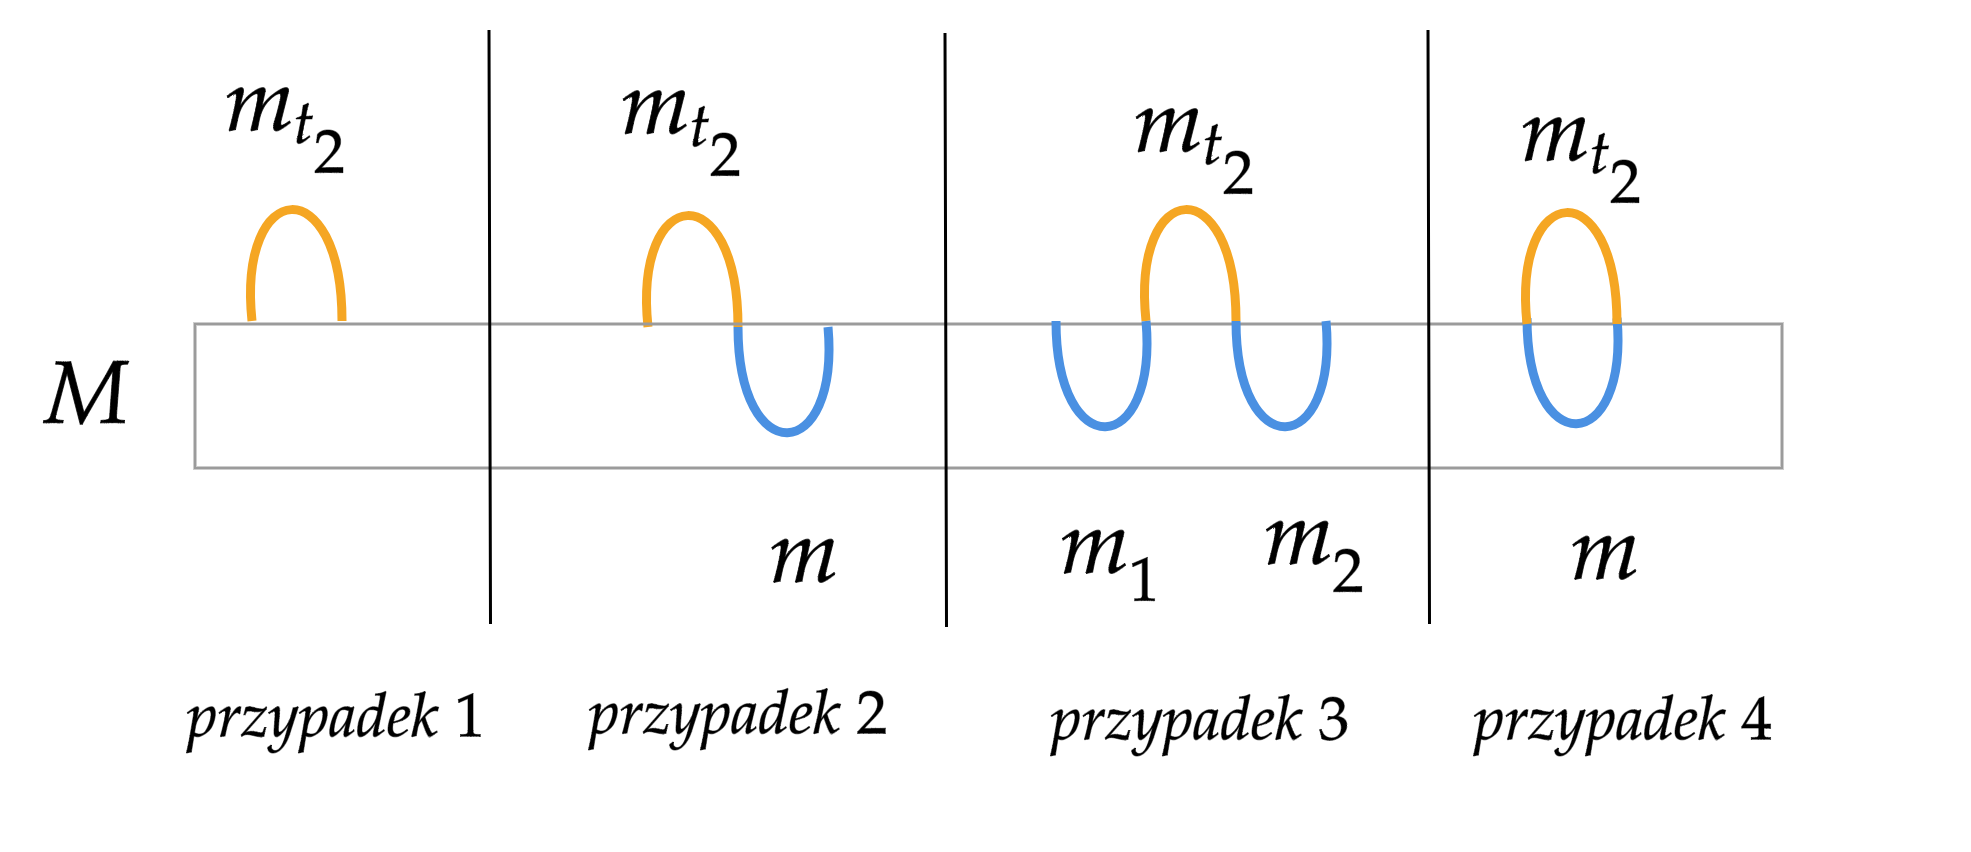
\includegraphics[width=16cm]{hamiltonian_merge2.png}
\caption{Dodawanie nowej krawędzi $m_{t_2}$ do skojarzenia $M$.}
\end{figure}

\texttt{SCALAJĄCY} - zauważmy, że scalane $F_{t_1}$ oraz $F_{t_2}$ nie mają wspólnych krawędzi, jedynie wierzchołki. Z powyższego wynika, że dla każdego wierzchołka $u$ należącego do $X_t$: $deg_t(u) = deg_{t_1}(u) + deg_{t_2}(u)$. Zauważmy, że musi być spełniony warunek $deg_t(u) \leq 2$. Jeśli $\mathcal{D}_{t_1}$ i $\mathcal{D}_{t_2}$ nie spełniają tego warunku, nie rozpatrujemy ich. Jednakże nie jest to warunek wystarczający, by rozwiązanie częściowe w kubełku $t$ było poprawne. Może się zdarzyć (jak przy dodawaniu krawędzi), że scalanie utworzy nam cykl. Scalając $M_{t_1}$ i $M_{t_2}$ uzupełniamy nasze obecne $M$ najpierw skojarzonymi wierzchołkami $m_{t_1} \in M_{t_1}$, by następnie pojednczo dodawać $m_{t_2} \in M_{t_2}$. Dla każdego nowo dodawanego $m_{t_2} = \{u, w\}$, sprawdzamy wszystkie $m \in M$, rozważając następujące przypadki (zobrazowane na rys. \ref{hamiltonian_merge}):
\begin{enumerate}
\item $\forall_{m \in M}: m_{t_2} \cap m = \emptyset$, do skojarzenia $M$ dorzucamy $m_{t_2}$.
\item $\exists_{m = \{v, z\} \in M}: \abs{m_{t_2} \cap m} = 1 \wedge \forall_{m^{\prime} \in M, m^{\prime} \ne m}: m_{t_2} \cap m^{\prime} = \emptyset$ - bez straty ogólności załóżmy, że $u = v$, czyli $m_{t_2} \cap m = \{u\}$, z $M$ usuwamy $m$ i dorzucamy nowe skojarzenie $\{w, z\}$.
\item $\exists_{m_1 = \{v_1, z_1\} \in M}: \abs{m_{t_2} \cap m_1} = 1 \wedge \exists_{m_2 = \{v_2, z_2\} \in M, m_2 \ne m_1}: \abs{m_{t_2} \cap m_2} = 1$ - bez straty ogólności załóżmy, że $u = v_1$ i $w = v_2$ (istotnym spostrzeżeniem jest fakt, że $m_{t_2} \cap m_1 \ne m_{t_2} \cap m_2$), usuwamy $m_1$ i $m_2$ z $M$ oraz dodajemy nowe skojarzenie $\{z_1, z_2\}$.
\item $\exists_{m \in M}: \abs{m_{t_2} \cap m} = 2$ - \texttt{CYKL}, $M_{t_1}$ i $M_{t_2}$ nie utworzą nam poprawnego rozwiązania.
\end{enumerate}

Końcowy wynik dla trójki $(t, \mathcal{D}, M)$ jest alternatywą po wszystkich $(t_1, \mathcal{D}_{t_1}, M_{t_1})$ i $(t_2, \mathcal{D}_{t_2}, M_{t_2})$, które spełniają wyżej wymienione warunki:

$$c[t][\mathcal{D}][M] = \bigvee \limits_{\mathcal{D}_{t_1}, \mathcal{D}_{t_2}, M_{t_1}, M_{t_2}} c[t_1][\mathcal{D}_{t_1}][M_{t_1}] \wedge c[t_2][\mathcal{D}_{t_2}][M_{t_2}]$$

Dla każdego kubełka mamy nie więcej niż $3^k \cdot k^k$ stanów. Zatem złożoność czasowa standardowego algorytmu dynamicznego po dekompozycji drzewowej dla problemu istnienia cyklu Hamiltona wynosi $k^{\Omicron(k)} \cdot n$, gdzie $n$ jest liczbą wierzchołków grafu $G$ danego na wejściu. 

\newpage
  	\chapter{Algorytmy dynamiczne z zastosowaniem techniki Cut \& Count}

W poprzednim rozdziale zostały przedstawione klasyczne algorytmy dynamiczne po dekompozycji drzewowej dla dwóch problemów decyzyjnych: drzewa Steinera oraz cyklu Hamiltona. Złożoność czasowa obu tych algorytmów jest niesatysfakcjonująca, gdyż zależy od $k^{\Omicron{(k)}}$ (gdzie $k$ jest szerokością drzewową). Czynnik ten jest następstwem trzymania odpowiednio: wszystkich możliwych podziałów cząstkowego drzewa Steinera na spójne poddrzewa oraz wszystkich możliwych skojarzeń wierzchołków wiszących w pary reprezentujące ścieżki będące częścią szukanego cyklu Hamiltona. W tym rodziale przedstawię dynamiczne algorytmy randomizowane (po dekompozycji drzewowej), bazujące na technice Cut \& Count opublikowanej w \cite{parametrized_algorithms}, która znosi konieczność śledzenia podziału na partycje czy skojarzenia, tym samym znacznie poprawiając złożoność czasową w stosunku do klasycznych algorytmów dynamicznych. Technika Cut \& Count redukuje problemy decyzyjne do problemów zliczania wszystkich możliwych rozwiązań modulo $2$, jednocześnie dopuszczając rozwiązania niespójne (las w przypadku drzewa Steinera, zbiór cykli w przypadku cyklu Hamiltona). Technika Cut \& Count bazuje na tymczasowym poluzowywaniu ograniczeń dotyczących spójności szukanych rozwiązań, z tego względu znajduje ona uniwersalne zastosowanie tylko do problemów o spójnych rozwiązaniach. Niech $\mathcal{S} \subset 2^U$ będzie zbiorem szukanych rozwiązań, a $U$ naszym uniwersum (zazwyczaj jest to zbiór wierzchołków lub krawędzi grafu danego na wejściu). Pytamy, czy $\mathcal{S}$ jest pusty. Na technikę Cut \& Count składają się dwa kroki:

\begin{enumerate}

\item[Cut] - poluzuj wymagania dotyczące spójności szukanego rozwiązania, tj. na tym etapie dopuszczamy rozwiązania niespójne należące do zbioru $\mathcal{R} \supseteq \mathcal{S}$. Ponadto rozważamy zbiór $\mathcal{C}$ składający się z par $(X, C)$, gdzie $X \in \mathcal{R}$ a $C$ jest partycją podzbioru wierzchołków grafu wejściowego $(V_1, V_2)$, z którą $X$ jest kompatybilny (żadna spójna składowa nie ma niepustego przecięcia zarówno z $V_1$, jak i $V_2$).  

\item[Count] - wyizoluj jedno z możliwych rozwiązań (o ile takie istnieje) poprzez przypisanie loswych wag elementom z uniwersum $U$. Rozbij zbiór $\mathcal{C}$ ze względu na wagi $w = w(X)$, a następnie oblicz parzystości zbiorów $\abs{\mathcal{C}_w}$ używając formuł rekurencyjnych. To pozwoli odrzucić wszystkie niepoprawne rozwiązania (niespójne), tj. $X \in \mathcal{R} \setminus \mathcal{S}$, ponieważ każde niespójne rozwiązanie jest kompatybilne z parzystą ilością partycji. Istnienie spójnego, wyizolowanego rozwiązania sprawi, że jedna z wartości $\abs{\mathcal{C}_w}$ będzie równa $1$.

\end{enumerate}

    	\section{Drzewo Steinera}
Podobnie jak w poprzednim rozdziale, mamy dany graf $G$ wraz ze zbiorem terminali $K \subseteq V(G)$ oraz jego dekompozycję drzewową $\mathcal{T} = (T, \{X_t\}_{t \in V(T)})$. Dodatkowo dostajemy liczbę naturalną $\ell$. Pytamy, czy istnieje drzewo Steinera o rozmiarze co najwyżej $\ell$, innymi słowy: czy istnieje spójny graf acykliczny łączący wszystkie terminale, o co najwyżej $\ell$ krawędziach. Dążymy do udowodnienia następującego twierdzenia:

\begin{theorem}
\label{monte_carlo}
Istnieje algorytm Monte Carlo z jednostronnym błędem (odpowiedź fałszywie negatywna), który rozwiązuje problem drzewa Steinera w czasie $3^k \cdot n^{\Omicron(1)}$ mając na wejściu daną dekompozycję drzewową grafu o szerokości drzewowej $k$.
\end{theorem}

\begin{proof}
Jak już zostało wspomniane, sprowadzamy problem decyzyjny do problemu parzystości ilości poprawnych, spójnych rozwiązań. Jednakże nie liczymy jej bezpośrednio, a uwzględniając rozwiązania niespójne - jak zostanie to pokazane, każde z nich wliczamy do końcowego wyniku parzystą liczbę razy, dzięki czemu wynik końcowy jest poprawny.

Powołując się na \cite{parametrized_algorithms}, zdefiniujmy dwa zbiory - $\mathcal{R}$ niech będzie zbiorem ,,lasów Steinera'', tj. zbiorem acyklicznych podgrafów $G$, które sumarycznie składają się z co najwyżej $\ell$ krawędzi i zawierają $K$, $\mathcal{S}$ niech zawiera te podgrafy z $\mathcal{R}$, które są dodatkowo spójne, innymi słowy $\mathcal{S}$ składa się z drzew Steinera:

$$\mathcal{R} = \{H \subseteq G: \abs{E(H)} \leq \ell, K \subseteq V(H)\}$$
$$\mathcal{S} = \{H \in \mathcal{R}: H\ jest\ sp\mbox{ó}jny\}$$

Chcemy, by każdy element z $\mathcal{R} \setminus \mathcal{S}$ został zliczony parzystą liczbę razy, natomiast każdy element ze zbioru $\mathcal{S}$ nieparzystą liczbę razy. W tym celu definiujemy rodzinę przecięć, które są podziałami $V(H)$ na dwa podzbiory $V^1$ i $V^2$. Mówimy, że podgraf $H$ grafu $G$ jest kompatybilny z przecięciem $(V^1, V^2)$, jeśli żadna z krawędzi $H$ nie ma końców po obu stronach przecięcia, tj. wtedy gdy $E(H) \subseteq {V^1 \choose 2} \cup {V^2 \choose 2}$, gdzie ${X \choose 2}$ oznacza wszystkie dwuelementowe podzbiory zbioru $X$.  

Zastanówmy się, jak wiele przecięć jest komptybilnych z danym grafem $H$. Skoro żadna z krawędzi nie może być rozpięta pomiędzy $V^1$ i $V^2$, każdy spójny komponent $H$ musi być w całości w $V^1$ lub w $V^2$. Z powyższego dostajemy, że dla danego $H$ mamy $2^c$ kompatybilnych przecięć, gdzie $c$ jest liczbą spójnych składowych $H$. Prawie mamy już to, co chcieliśmy - każde niespójne $H$ (z więcej niż jedną spójną składową) jest kompatybilne z parzystą liczbą przecięć. Niestety spójne rozwiązania są również kompatybilne z parzystą liczbą przecięć, a precyzując - każde z dokładnie dwoma. Możemy to naprawić, wybierając dowolny wierzchołek $v_1 \in K$ i przypisać go na stałe tylko do $V^1$. Zapiszmy formalnie definicję przecięć kompatybilnych z $H$:

$$\texttt{cuts} (V(H), v_1) \coloneqq \{(V^1, V^2): V^1 \cup V^2 = V(H) \wedge V^1 \cap V^2 = \emptyset \wedge v_1 \in V^1\}$$

Pokażmy teraz, że zamiast liczyć parzystość $\abs{\mathcal{S}}$, możemy policzyć parzystość zbioru składającego się z podzbiorów należących do $\mathcal{R}$ wraz z wszystkimi kompatybilnymi do nich przecięciami:

$$\mathcal{C} = \{(H, (V^1, V^2)) \in \mathcal{R} \times \texttt{cuts}(V(H), v_1) : H\ jest\ kompatybilny\ z\ (V^1, V^2)\}$$

\begin{lemma}
Parzystość $\abs{\mathcal{C}}$ jest równa parzytości $\abs{\mathcal{S}}$.
\end{lemma}

\begin{proof}
Rozważmy graf $H$ należący do $\mathcal{R}$, który ma $c$ spójnych składowych. Każda spójna składowa musi się znaleźć w całości w $V^1$ albo w $V^2$, wpp. mielibyśmy krawędź przechodzącą przez przecięcie. Jednakże spójna składowa zawierająca $v_1$ może się znaleźć tylko po stronie $V^1$. Z tego powodu $H$ jest kompatybilny z $2^{c-1}$ przecięciami. Dla $H \in \mathcal{S}$ liczba ta jest nieparzysta, natomiast dla $H \in \mathcal{R} \setminus \mathcal{S}$ parzysta. 
\end{proof}

Wobec powyższego lematu, pozostaje pokazać algorytm obliczania parzystości $\mathcal{C}$. Okazuje się, że możemy to zrobić bez spamiętywania wszystkich dotychczasowo poprawnych stanów rozwiązań cząstkowych, tj. bez ich podziałów na partycje. Dzięki temu dostaniemy algorytm o złożoności $2^{\Omicron(k)}$.

Dla każdego kubełka $t \in V(T)$, liczby naturalnej $i \leq l$ i funkcji $f: X_t \to \{0,1,2\}$ obliczamy $c[t][f][i]$ będące liczbą par $(H, (V^1, V^2))$, takich że:

\begin{enumerate}
\item $H$ jest podgrafem $(V_t, E_t)$ o dokładnie $i$ krawędziach oraz $H$ zawiera wszystkie terminale dotychczasowo wprowadzone w bieżącym poddrzewie, tj. $K \cap V_t$
\item $(V^1, V^2)$ jest przecięciem kompatybilnym z $H$, tj. $V^1 \cup V^2 = V(H)$, $V^1 \cap V^2 = \emptyset$, $v_1 \notin V^2$
\item przecięcie $H$ z wierzchołkami należącymi do kubełka $t$ jest równe $V(H) \cap X_t = f^{-1}(1) \cup f^{-1}(2)$
\item funkcja $f$ opisuje przynależność wierzchołków ze zbioru $X_t \setminus f^{-1}(0)$ do $V^1$ i $V^2$, tj. $V^j \cap V(H) \cap X_t = f^{-1}(j)$ gdzie $j \in \{1,2\}$
\end{enumerate} 

Zanim przejdę do rekurencyjnych formuł obliczania wartości $c[t][f][i]$, pokażę w jaki sposób problem parzystości $\mathcal{C}$ redukuje się do problemu istnienia drzewa Steinera. Oczywistym jest, że mogą istnieć dwa różne (parzyście wiele różnych) drzewa Steinera o tej samej liczbie krawędzi. Problem ten rozwiążemy poprzez wprowadzenie wag na krawędziach grafu $G$, które pozwolą nam rozróżniać poszczególne rozwiązania. 
Dla odpowiednio dużego $N$, losowo (niezależnie i z równym prawdopodobieństwem) wybieramy wagi ze zbioru $\{1,2,\dots,N\}$ i przyporządkowywujemy je krawędziom należącym do $E(G): \mathbf{w}(e) \in \{1,2,\dots,N\}$. Zdefiniujmy wagę podgrafu $H$ następująco $\mathbf{w}(H) = \sum_{e \in E(H)} \mathbf{w}(e)$. Dla liczby naturalnej $w$, niech $\mathcal{R}_w = \{H \in \mathcal{R} : \mathbf{w}(H) = w\}$. Podobnie definiujemy $\mathcal{S}_w$ i $\mathcal{C}_w$. Z oczywistych względów $\abs{\mathcal{S}_w} \mod 2 = \abs{\mathcal{C}_w} \mod 2$. Intuicyjnie, wystarczająco duże $N$ powinno porozrzucać poprawne rozwiązania do różnych $\mathcal{S}_w$, dzięki czemu implikacja $\exists_{w} :\abs{\mathcal{S}_w} \mod 2 = 1 \implies$ $istnieje$ $drzewo$ $Steinera$ $o$ $i \leq l$ $kraw\mbox{ę}dziach$ z wysokim prawdopodobieństwem zachodzi w obie strony. Autorzy udowadniają za pomocą tzw. lematu izolującego coś znacznie silniejszego - mianowicie wystarczy wziąć $N = \Omega(\abs{E(G)})$, żeby ze stałym prawdopodobieństwem otrzymać co najmniej jeden zbiór $\mathcal{S}_w$ rozmiaru dokładnie $1$.

\begin{definition}
Funkcja $\mathbf{w}: U \to \mathbb{Z}$ izoluje rodzinę zbiorów $\mathcal{F} \subseteq 2^U$ jeśli istnieje unikalne $S' \in \mathcal{F}$, takie że $\mathbf{w}(S') = min_{S \in \mathcal{F}} \mathbf{w}(S)$. W naszym przypadku $\mathbf{w}(X) = \sum_{u \in X} \mathbf{w}(u)$.
\end{definition}

\begin{lemma}[Lemat izolujący]
Niech $\mathcal{F} \subseteq 2^U$będzie rodziną zbiorów w uniwersum $U$, gdzie $\abs{\mathcal{F} > 0}$. Dla każdego $u \in U$, wybieramy $\mathbf{w}(u) \in \{1, 2, \ldots, N\}$ z jednakowym prawdopodobieństwem, niezależnie. Wtedy
$$Pr(\mathbf{w} \ izoluje \ \mathcal{F}) \geq 1 - \frac{\abs{U}}{N}$$
\end{lemma}

\begin{proof}
Niech $u \in U$ będzie dowolnym elementem z uniwersum $U$, który znajduje się w co najmniej jednym zbiorze z $\mathcal{F}$ i w co najmniej jednym z nich się nie pojawia - taki element nie musi istnieć. Definiujemy:
$$\alpha(u) = min_{S \in \mathcal{F}, u \notin S} \mathbf{w}(S) - min_{S \in \mathcal{F}, u \in S} \mathbf{w}(S \setminus \{u\})$$

Zauważmy, że $\alpha(u)$ jest niezależne od $\textbf{w}(u)$. Dostajemy, że
\begin{equation}
\label{pr}
Pr(\alpha(u) = \mathbf{w}(u)) \leq \frac{1}{N},
\end{equation}
ponieważ wagę $\mathbf{w}(u)$ możemy wylosować na sam koniec, kiedy wszystkie inne wagi są już ustalone.
Załóżmy, że mamy dwa zbiory $A, B \in \mathcal{F}$ o minimalnej wadze. Musi je rozróżniać co najmniej jeden element, tzn. istnieje $x \in A \setminus B$. Dostajemy
$$\alpha(x) = min_{S \in \mathcal{F}, x \notin S} \mathbf{w}(S) - min_{S \in \mathcal{F}, x \in S} \mathbf{w}(S \setminus \{x\})$$
$$= \mathbf{w}(B) - (\mathbf{w}(A) - \mathbf{w}(x))$$
$$= \mathbf{w}(x)$$
Jesli $W$ nie izoluje $\mathcal{F}$, wtedy istnieje element $x$ i zbiory $A, B \in \mathcal{F}$ takie że $x \in A \setminus B$ i $\alpha(x) = \mathbf{w}(x)$. Jednakże na podstawie \ref{pr}, to się zdarza z prawdopodobieństwem nie większym niż $\frac{\abs{U}}{N}$.
\end{proof}

Naszym uniwersum są krawędzie grafu wejściowego $G$ ($U = E(G)$), natomiast $\mathcal{F} = \{E(H) : H \in S\}$. Wagi na krawędziach losujemy ze zbioru $\{1,2, \ldots, 2 \abs{U}\}$, a następnie liczymy parzystość ilości rozwiązań dla poszczególnych $\mathcal{C}_w$. Musimy nieznacznie zmodyfikować, dla jakich parametrów liczymy rozwiązania cząstkowe $c[t][f][i]$ wspomniane powyżej. tj. dorzucamy jeszcze jeden parametr $w$ i liczymy, ile jest podgrafów $H$ o wadze $w$, $i$ krawędziach, kompatybilnych z podziałem $(V_1, V_2)$. Poniżej przedstawiam rekurencyjne formuły zależne od typu kubełka $t$. Rozwiązanie końcowe zależy od tego, czy istnieje $i \leq l$ oraz $w  \leq 2\abs{E}l$, dla których  $c[r][0][i][w] \mod 2 = 1$. Jeśli tak, to istnieje drzewo Steinera o $i$ krawędziach. Jeśli nie, to z prawdopodobieństwem co najmniej $\frac{1}{2}$ nie istnieje drzewo Steinera o co najwyżej $l$ krawędziach. 
\newline\newline
\texttt{LIŚĆ u} - dla wszystkich liści $c[t][\emptyset][0][0] = 1$, ponieważ $H$ nie ma jeszcze wprowadzonych żadnych wierzchołków ani krawędzi.
\newline\newline
\texttt{WPROWADZAJĄCY u} - zauważmy, że $u \in K \implies f(u) \neq 0$ oraz $u = v_1 \implies f(u) = 1$. Jeśli któryś z wymienionych warunków nie jest spełniony $c[t][f][i][w] = 0$, wpp.

$$c[t][f][i][w] = c[t^{\prime}][f_{\big|X_{t^{\prime}}}][i][w]$$
\newline\newline
\texttt{ZAPOMINAJĄCY u} - dla kubełka zapominającego dodajemy wyniki cząstkowe przyjmując, że w dziecku wierzchołek $u$ mógł mieć odpowiednio przypisane wartości funkcji $f(u)$: $0$, $1$, $2$.
\[
c[t][f][i][w] =  
  \begin{tabular}{ccc}
  $\ \ c[t^{\prime}][f \cup \{u\} \to \{0\}][i][w]$\\
  $+ c[t^{\prime}][f \cup \{u\} \to \{1\}][i][w]$\\
  $+ c[t^{\prime}][f \cup \{u\} \to \{2\}][i][w]$
  \end{tabular}
\]
\newline\newline
\texttt{UZUPEŁNIAJĄCY uv} - zauważmy, że dla kubełka uzupełniającego $uv$ musi zachodzić $f(u) = f(v) \neq 0$, ponieważ żadna krawędź nie może przechodzić przez przecięcie oraz wierzchołki izolowane ($f(u) = 0$) nie mogą być incydentne z jakąkolwiek krawędzią. Jeśli powyższe warunki nie są spełnione $c[t][f][i][w] = c[t^{\prime}][f][i][w]$, innymi słowy nie włączamy krawędzi $uv$ do bieżącego rozwiązania, wpp.

$$c[t][f][i][w] = c[t^{\prime}][f][i-1][w-w_{uv}]$$
\newline\newline
\texttt{SCALAJĄCY} - dla kubełka scalającego sumujemy po wszystkich parach rozwiązań cząstkowych, gdzie $w(H_1) + w(H_2) = w(H)$ oraz $\abs{E(H_1)} + \abs{E(H_2)} = \abs{E(H)}$

$$c[t][f][i][w] = \sum_{i_1 + i_2 = i, w_1 + w_2 = w} c[t_1][f][i_1][w_1] + c[t_2][f][i_2][w_2]$$

Złożoność powyższego algorytmu wynosi $3^k \cdot n^{\Omicron(1)}$, czyli zależność złożoności czasowej od szerokości drzewowej jest rzędu $2^{\Omicron(k)}$, a nie jak w przypadku standardowego algorytmu dynamicznego $k^{\Omicron(k)}$, co kończy dowód twierdzenia \ref{monte_carlo}.
\end{proof}

    	\section{Cykl Hamiltona}

Zastanówmy się, jak można zastosować technikę Cut \& Count w celu rozwiązania problemu istnienia cyklu Hamiltona (przedstawionego w poprzednim rozdziale) oraz jak bardzo pozwoli nam ona zbić złożoność czasową w stosunku do standardowego algorytmu po dekompozycji drzewowej. Ponieważ apekty techniczne w większości pokrywają się z tym, co zostało przedstawione w poprzednim paragrafie w kontekście drzewa Steinera, skupię się wyłącznie na różnicach, niuansach charakterystycznych dla cyklu Hamiltona.

Po pierwsze skupmy się na dopuszczalnych rozwiązaniach. Pominięcie wymogu spójności redukuje problem cyklu Hamiltona do problemu pokrycia wierzchołkowego grafu $k$ cyklami, gdzie w naszym przypadku $k \in \{1, \ldots, \floor*{\frac{|V|}{2}}\}$. Zbiór $\mathcal{R}$ zawiera wszystkie takie pokrycia $H$, które składają się z cykli zawierających co najmniej dwa wierzchołki oraz które sumarycznie pokrywają wszystkie wierzchołki grafu wejściowego $G$:

$$\mathcal{R} = \{H \subseteq G: V(H) = V(G), \forall u \in V(H): deg(u) = 2\}$$
$$\mathcal{S} = \{H \in \mathcal{R}: H\ jest\ sp\mbox{ó}jny\}$$

Po drugie zauważmy, że o ile w przypadku liczenia cząstkowych rozwiązań dla drzewa Steinera, mamy zachowany niezmiennik, że cząstkowe rozwiązanie składa się z drzew, o tyle w przypadku cyklu Hamiltona podobny niezmiennik nie zachodzi. Rozwiązanie dla bieżącego podgrafu $G_t$ niekoniecznie składa się z cykli, ponieważ może zawierać także ścieżki. Zliczamy takie rozwiązania, dopóki istnieje możliwość domknięcia wszystkich ścieżek (tzn. w wierzchołku \texttt{ZAPOMINAJĄCY u} wymagamy, by $deg(u) = 2$).

Zbiór $\mathcal{C}$ definiujemy podobnie jak dla drzewa Steinera, z dwiema drobnymi modyfikacjami. Jedna z nich dotyczy $v_1$, który dla cyklu Hamiltona jest dowolnym, ale ustalonym wierzchołkiem ze zbioru $V(G)$. Druga natomiast dotyczy podziału $(V^1, V^2)$, który definiujemy tylko na wierzchołkach o stopniu $1$.
$$\texttt{cuts} (V_{deg_1}(H), v_1) \coloneqq \{(V^1, V^2): V^1 \cup V^2 = V_{deg_1}(H) \wedge V^1 \cap V^2 = \emptyset \wedge v_1 \in V^1\}$$
$$\mathcal{C} = \{(H, (V^1, V^2)) \in \mathcal{R} \times \texttt{cuts}(V_{deg_1}(H), v_1) : H\ jest\ kompatybilny\ z\ (V^1, V^2)\}$$
\newline
Losowanie wag na krawędziach i definiowanie $\mathcal{R}_w$, $\mathcal{S}_w$ oraz $\mathcal{C}_w$ nie ulega zmianie. Jedyne nad czym musimy się pochylić, to jak trzymamy bieżący stan (tj. dla jakich parametrów wyliczamy wartości $c$) oraz jak definiujemy funkcje rekurencyjne.

\begin{figure}
\centering
\label{cnc_hamiltonian}
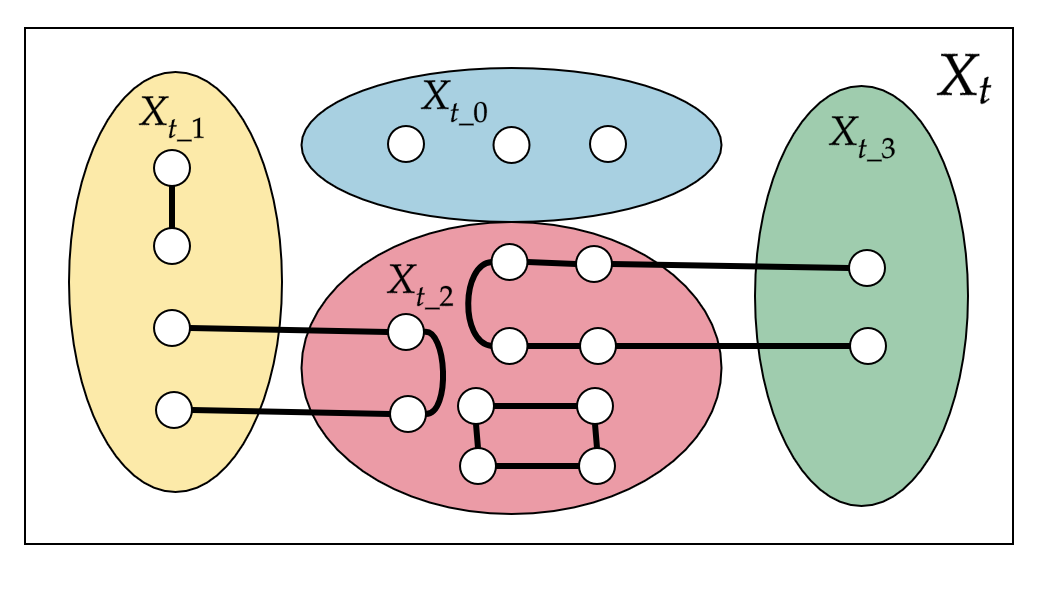
\includegraphics[width=16cm]{cnc_hamiltonian2.png}
\caption{Wizualizacja czterech stanów, w jakich mogą się znajdować wierzchołki z $X_t$.}
\end{figure}

Dla każdego kubełka $t \in V(T)$, funkcji $f: X_t \to \{0,1,2,3\}$ oraz wagi $w$ obliczamy $c[t][f][w]$ będące liczbą par $(H, (V^1, V^2))$, takich że:

\begin{enumerate}
\item $H$ jest podgrafem $(V_t, E_t)$ oraz $H$ zawiera wszystkie wierzchołki dotychczasowo wprowadzone w bieżącym poddrzewie, tj. $V(H) = V_t$
\item $(V^1, V^2)$ jest przecięciem kompatybilnym z $H$, tj. $V^1 \cup V^2 = V_{deg_1}(H)$, $V^1 \cap V^2 = \emptyset$, $v_1 \notin V^2$
\item przecięcie $H$ z wierzchołkami należącymi do kubełka $t$ jest równe $V(H) \cap X_t = X_t = f^{-1}(0) \cup f^{-1}(1) \cup f^{-1}(2) \cup f^{-1}(3)$
\item funkcja $f$ opisuje przynależność wierzchołków ze zbioru $X_t$ do podzbiorów $X_{t\_0}, X_{t\_1}, X_{t\_2}, X_{t\_3}$, tj. $X_{t\_j} \cap V(H) = f^{-1}(j)$, gdzie $j \in \{0,1,2,3\}$
\item $V^1 \cup V^2$ nie ma wierzchołków poza $X_t$, innymi słowy $V_{deg_1}(H) \cap X_t = V_{deg_1}(H)$, inaczej nieodwołalnie zostawilibyśmy niedomknięty cykl
\item $X_{t\_1} = V^1$ oraz $X_{t\_3} = V^2$
\item $u \in X_{t\_i} \implies deg(u) = i$ dla $i \in \{0,1,2\}$
\item $u \in X_{t\_3} \implies deg(u) = 1$
\item $\sum_{e \in E(H)} \mathbf{w}(e) = w$
\end{enumerate}
$$$$
Podsumowując, mamy cztery stany, które reprezentują wierzchołki $u \in X_t$, zostały one zobrazowane na rys. \ref{cnc_hamiltonian}: 
\begin{itemize}
\item[$X_{t\_0}$:] stan reprezentujący wierzchołki o stopniu $0$
\item[$X_{t\_1}$:] stan reprezentujący wierzchołki o stopniu $1$, które znalazły się po stronie $V^1$ przecięcia
\item[$X_{t\_3}$:] stan reprezentujący wierzchołki o stopniu $1$, które znalazły się po stronie $V^2$ przecięcia
\item[$X_{t\_2}$:] stan reprezentujący wierzchołki o stopniu $2$
\end{itemize}

Zauważmy, że każdy wierzchołek musi przechodzić przez następujące stany $0 \to \{1 \ lub \ 3\} \to 2$ (wyjątkiem jest $v_1$, które nigdy nie będzie należało do $X_{t\_3}$). Poniżej przedstawiam definicje rekurencyjne obliczania wartości $c[t][f][w]$. Algorytm zwraca, że istnieje cykl Hamiltona, jeśli $\exists_{w \leq nN}: c[r][0][w] \mod 2 = 1$, gdzie $r$ jest korzeniem dekompozycji drzewowej, a $n = \abs{V(G)}$.
\newline\newline
\texttt{LIŚĆ u} - dla wszystkich liści $c[t][\emptyset][0] = 1$
\newline\newline
\texttt{WPROWADZAJĄCY u} - wierzchołek $u$ w momencia wprowadzania nie jest incydentny z żadną krawędzią, zatem jeśli $f(u) \neq 0$, to $c[t][f][w] = 0$, wpp.
$$c[t][f][w] = c[t^{\prime}][f_{\big|X_{t^{\prime}}}][i][w]$$
\newline
\texttt{ZAPOMINAJĄCY u} - wierzchołek może zostać zapomniany wtw. gdy znajduje się w $X_{t_2}$, czyli ma dwie incydentne krawędzie, jeśli $f(u) \neq 2$, to $c[t][f][w] = 0$, wpp.
$$c[t][f][w] = c[t^{\prime}][f \cup \{u\} \to \{2\}][w]$$
\newline

\begin{table}
\centering
\label{add_edge_table}
\begin{tabular}{c|c|c|c|c}
 & $X_{t^{\prime}\_0}$ & $X_{t^{\prime}\_1}$ & $X_{t^{\prime}\_2}$ & $X_{t^{\prime}\_3}$ \\
\hline
$X_{t^{\prime}\_0}$ & $(1,1) \vee (3,3)$ & $(1,2)$ & $\emptyset$ & $(3,2)$ \\
\hline
$X_{t^{\prime}\_1}$ & $(2,1)$ & $(2,2)$ & $\emptyset$ & $\emptyset$ \\
\hline
$X_{t^{\prime}\_2}$ & $\emptyset$ & $\emptyset$ & $\emptyset$ & $\emptyset$ \\
\hline
$X_{t^{\prime}\_3}$ & $(2,3)$ & $\emptyset$ & $\emptyset$ & $(2,2)$ \\
\end{tabular}
\caption{Możliwe zmiany stanu w przypadku dodawania krawędzi. Tabelę należy rozumieć w następujący sposób: $tab[f^{\prime}(u)][f^{\prime}(v)] = (f(u), f(v))$, $i$ jest tożsame z $X_{t\_i}$.}
\end{table}
$$$$
\texttt{UZUPEŁNIAJĄCY uv} - po pierwsze możemy nie dodwać krawędzi $uv$ do rozwiązania, wtedy $c[t][f][w] = c[t^{\prime}][f][w]$. Zastanówmy się, jakie warunki muszą być spełnione, żeby można było wstawić krawędź $uv$:
\begin{itemize}
\item $deg(u) < 2$ oraz $deg(v) < 2$
\item oba wierzchołki były/są po tej samej stronie przecięcia $(V^1, V^2)$.
\item tabela \ref{add_edge_table} pokazuje jakie są możliwe zmiany stanu w przypadku dodawania krawędzi. Tabelę należy rozumieć w następujący sposób: $tab[f^{\prime}(u)][f^{\prime}(v)] = (f(u), f(v))$, $i$ jest tożsame z $X_{t\_i}$.
\end{itemize}

\[
c[t][f][w] =  
\left \{
  \begin{tabular}{ccc}
  jeśli spełnione są powyższe warunki \\
  oraz \\
  $f(u)$, $f(v)$, $f^{\prime}(u)$ i  $f^{\prime}(v)$ są w relacji opisanej za pomocą tabeli \ref{add_edge_table} \\  
  $c[t^{\prime}][f^{\prime}][w - w_{uv}]$,\\
  wpp. $0$
  \end{tabular}
\right. 
\]

\begin{table}
\centering
\label{merge_table}
\begin{tabular}{c|c|c|c|c}
 & $X_{t_2\_0}$ & $X_{t_2\_1}$ & $X_{t_2\_2}$ & $X_{t_2\_3}$ \\
\hline
$X_{t_1\_0}$ & $0$ & $1$ & $2$ & $3$ \\
\hline
$X_{t_1\_1}$ & $1$ & $2$ & $-$ & $-$ \\
\hline
$X_{t_1\_2}$ & $2$ & $-$ & $-$ & $-$ \\
\hline
$X_{t_1\_3}$ & $3$ & $-$ & $-$ & $2$ \\
\end{tabular}
\caption{Zmiana stanu wierzchołka po scaleniu dwóch cząstkowych rozwiązań. Tabelę należy interpretować następująco: $tab[f_1(u)][f_2(u)] = f(u)$, $i$ jest tożsame z $X_{t\_i}$.}
\end{table}
$$$$
\texttt{SCALAJĄCY} - podobnie jak w przypadku dodawania krawędzi, aby scalanie dwóch cząstkowych rozwiązań było możliwe, muszą być spełnione następujące wymagania:
\begin{itemize}
\item $deg_{t_1}(u) + deg_{t_2}(u) \leq 2$, dla każdego $u \in X_t$
\item jeśli $u \in X_{t_1\_1}$, to $u \notin X_{t_2\_3}$, dla każdego $u \in X_t$ ($u$ nie może być po dwóch różnych stronach przecięcia)
\item tabela \ref{merge_table} pokazuje, jak zmienia się stan $u$ po scaleniu dwóch cząstkowych rozwiązań. Tabelę należy interpretować następująco: $tab[f_1(u)][f_2(u)] = f(u)$, $i$ jest tożsame z $X_{t\_i}$.
\end{itemize}

\[
c[t][f][w] =  
\left \{
  \begin{tabular}{ccc}
  jeśli spełnione są powyższe warunki \\
  oraz $\forall u \in X_t$\\
  $f(u)$, $f_1(u)$ i $f_2(u)$ są w relacji opisanej za pomocą tabeli \ref{merge_table} \\  
  $\sum_{w_1 + w_2 = w} c[t_1][f_1][w_1] + c[t_2][f_2][w_2]$,\\
  wpp. $0$
  \end{tabular}
\right. 
\]

Złożoność powyższego algorytmu wynosi $4^k \cdot n^{\Omicron(1)}$, czyli zależność złożoności czasowej od szerokości drzewowej jest rzędu $2^{\Omicron(k)}$, a nie jak w przypadku standardowego algorytmu dynamicznego $k^{\Omicron(k)}$.

\newpage
	\begin{thebibliography}{9}
		\bibitem{kloks} 
			T. Kloks. 
			\textit{Treewidth. Computations and approximations}. 
			Lecture Notes in Computer Science, 842, 1994.
 
		\bibitem{bodlaender}  
			H. L. Bodlaender. 
			\textit{A linear-time algorithm for finding tree-decompositions of small treewidth}. 
			SIAM J. Comput. 25:6 (1996) 1305-1317
			
		\bibitem{robertson&seymour} 
			N. Robertson and P. D. Seymour. 
			\textit{Graph Minors II. Algorithmic aspects of treewidth}. 
			J. Algorithms 7 (1986) 309-322
			
		\bibitem{parametrized_algorithms}
			M. Cygan, F. V. Fomin, Ł. Kowalik, D. Lokshtanov, D. Marx, M. Pilipczuk, M. Pilipczuk, S. Saurabh
 			\textit{Parameterized Algorithms}.
 			
		\bibitem{knuthwebsite} 
			Knuth: Computers and Typesetting,
			\\\texttt{http://www-cs-faculty.stanford.edu/\~{}uno/abcde.html}
	\end{thebibliography} 



\end{document}
